\documentclass[12pt, openany, oneside]{book}

\usepackage{listings}
\usepackage[dvipsnames]{xcolor}
\usepackage{ctex}
\usepackage{fontspec}
\usepackage{setspace}
\usepackage{tikz}
\usepackage{anyfontsize}
\usepackage{sectsty}
\usepackage{titlesec}
\usepackage{float}
\usepackage[hidelinks]{hyperref}
\usepackage[a4paper]{geometry}
\usepackage{url}
\usepackage{amssymb}
\usepackage{fontawesome5}
\usepackage[most]{tcolorbox}
\usepackage{stackengine}
\usepackage{multirow}
\usepackage[T1]{fontenc}
\usepackage{diagbox}
\usepackage{longtable}
\usepackage{newtxtt}
\usepackage{pgf-umlcd}
\usepackage{bbding}
\usepackage[edges]{forest}

\usetikzlibrary{calc,trees,positioning,arrows,fit,shapes}
\usetikzlibrary{shapes.multipart,chains}
\usetikzlibrary{automata}
\usetikzlibrary{shadows}
\usetikzlibrary{arrows.meta}
\usetikzlibrary{matrix,backgrounds}

\makeatletter
\newcommand{\verbatimfont}[1]{\renewcommand{\verbatim@font}{\ttfamily#1}}
\makeatother

\def\rlwd{.5pt} \def\rlht{2.2ex} \def\rldp{.5ex}
\def\mydiv#1{~
  \rule[-\rldp]{\rlwd}{\rlht}
  \setbox0=\hbox{~#1}
  \stackunder[\dimexpr\rldp-\rlwd]{~#1}{\rule{\wd0}{\rlwd}}%
}

\definecolor{mycolor}{RGB}{0,128,128}
\newtcbox{\mybox} {
    on line,
    colback=mycolor,
    fontupper=\bfseries\color{white},
    boxrule=0pt,
    arc=5pt, 
    boxsep=0pt, 
    left=2pt, 
    right=2pt, 
    top=5pt, 
    bottom=5pt
}

\tikzset{block/.style={
        font=\sffamily,
        draw=black,
        thin,
        fill=pink!50,
        rectangle split,
        rectangle split horizontal,
        rectangle split parts=#1,
        outer sep=0pt},
        gblock/.style={
            block,
            rectangle split parts=#1,
            fill=green!30}
        }

\tikzstyle{ptr}  = [draw, -{Stealth[scale=1.0]}, blue]
\tikzstyle{head} = [rectangle, draw, text height=3mm, text width=3mm,
                    text centered, node distance=3cm, inner sep=0pt]
\tikzstyle{data} = [rectangle split, rectangle split parts=2, draw,
                    text centered, minimum height=3em]
\newcommand{\data}{
  data \nodepart{second}
  \phantom{\texttt{NULL}}
}

\tikzset{
    queue element/.style={
        draw,very thin,rounded corners,
        fill=yellow!30,
        minimum width=1cm,minimum height=.5cm,
        font=\sffamily\footnotesize
    },
    >={[scale=0.8]Triangle},
    queue/.style={matrix of nodes,
        nodes in empty cells,
        nodes={queue element, anchor=center},
        fill=green!20,
        column sep=5mm,
        row sep=2mm,
    },
}

\makeatletter
\def\BState{\State\hskip-\ALG@thistlm}
\makeatother

\tikzstyle{startend} = [rectangle, rounded corners, minimum width=3cm, minimum height=1cm, text centered, draw=black, fill=red!30]
\tikzstyle{io}        = [trapezium, trapezium left angle=70, trapezium right angle=110, minimum width=3cm, inner xsep = -15pt, minimum height=1cm, text centered, draw=black, fill=blue!30]
\tikzstyle{process}   = [rectangle, minimum width=3cm, minimum height=1cm, inner ysep=0, text centered, draw=black, fill=orange!30]
\tikzstyle{decision}  = [diamond,shape aspect=2.5, minimum width=3cm, minimum height=1cm, inner xsep=0,text centered, draw=black, fill=green!30]
\tikzstyle{arrow}     = [thick,->,>=stealth]

\setstretch{1.5}
\setlength{\parindent}{0cm}

\geometry{a4paper,top=2.5cm,bottom=2.5cm}

\titleformat{\chapter}{\Huge\Huge\bfseries}{\chaptertitlename\ \thechapter{\ }}{0pt}{\Huge}{}
\titlespacing{\chapter}{0pt}{0pt}{12pt}

\definecolor{dkgreen}{rgb}{0,0.4,0}
\definecolor{gray}{rgb}{0.5,0.5,0.5}
\definecolor{mauve}{rgb}{0.58,0,0.82}
\definecolor{LightGray}{gray}{0.9}

\lstset{
    basicstyle=\linespread{1.3} \fontspec{Consolas},    %  the size of the fonts that are used for the code
	basewidth=0.5em,
    numbers=left,            % where to put the line-numbers
    numberstyle=\color{black},  % the style that is used for the line-numbers
    numbersep=10pt,                  % how far the line-numbers are from the code
    backgroundcolor=\color{white},
    showspaces=false,
    showstringspaces=false,
    showtabs=false,
    frame=single,                   % adds a frame around the code
    rulecolor=\color{black},        % if not set, the frame-color may be changed on line-breaks within not-black text (e.g. commens (green here))
    tabsize=4,                      % sets default tabsize to 2 spaces
    captionpos=t,                   % sets the caption-position to bottom
    breaklines=false,                % sets automatic line breaking
    breakatwhitespace=true,        % sets if automatic breaks should only happen at whitespace
    title=\lstname,                   % show the filename of files included with \lstinputlisting;
    % also try caption instead of title
    numberstyle=\color{black},		% line number color
    keywordstyle=\color{blue},          % keyword style
    commentstyle=\color{dkgreen},       % comment style
    stringstyle=\color{mauve},         % string literal style
    escapeinside={\%*}{*)},            % if you want to add LaTeX within your code
    morekeywords={*,...}               % if you want to add more keywords to the set
}

\begin{document}

\thispagestyle{empty}

\begin{tikzpicture}[overlay,remember picture]
	% Background color
	\fill[
		black!2]
	(current page.south west) rectangle (current page.north east);

	% Rectangles
	\shade[
		left color=Dandelion,
		right color=Dandelion!40,
		transform canvas ={rotate around ={45:($(current page.north west)+(0,-6)$)}}]
	($(current page.north west)+(0,-6)$) rectangle ++(9,1.5);

	\shade[
		left color=lightgray,
		right color=lightgray!50,
		rounded corners=0.75cm,
		transform canvas ={rotate around ={45:($(current page.north west)+(.5,-10)$)}}]
	($(current page.north west)+(0.5,-10)$) rectangle ++(15,1.5);

	\shade[
		left color=lightgray,
		rounded corners=0.3cm,
		transform canvas ={rotate around ={45:($(current page.north west)+(.5,-10)$)}}] ($(current page.north west)+(1.5,-9.55)$) rectangle ++(7,.6);

	\shade[
		left color=orange!80,
		right color=orange!60,
		rounded corners=0.4cm,
		transform canvas ={rotate around ={45:($(current page.north)+(-1.5,-3)$)}}]
	($(current page.north)+(-1.5,-3)$) rectangle ++(9,0.8);

	\shade[
		left color=red!80,
		right color=red!80,
		rounded corners=0.9cm,
		transform canvas ={rotate around ={45:($(current page.north)+(-3,-8)$)}}] ($(current page.north)+(-3,-8)$) rectangle ++(15,1.8);

	\shade[
		left color=orange,
		right color=Dandelion,
		rounded corners=0.9cm,
		transform canvas ={rotate around ={45:($(current page.north west)+(4,-15.5)$)}}]
	($(current page.north west)+(4,-15.5)$) rectangle ++(30,1.8);

	\shade[
		left color=RoyalBlue,
		right color=Emerald,
		rounded corners=0.75cm,
		transform canvas ={rotate around ={45:($(current page.north west)+(13,-10)$)}}]
	($(current page.north west)+(13,-10)$) rectangle ++(15,1.5);

	\shade[
		left color=lightgray,
		rounded corners=0.3cm,
		transform canvas ={rotate around ={45:($(current page.north west)+(18,-8)$)}}]
	($(current page.north west)+(18,-8)$) rectangle ++(15,0.6);

	\shade[
		left color=lightgray,
		rounded corners=0.4cm,
		transform canvas ={rotate around ={45:($(current page.north west)+(19,-5.65)$)}}]
	($(current page.north west)+(19,-5.65)$) rectangle ++(15,0.8);

	\shade[
		left color=OrangeRed,
		right color=red!80,
		rounded corners=0.6cm,
		transform canvas ={rotate around ={45:($(current page.north west)+(20,-9)$)}}]
	($(current page.north west)+(20,-9)$) rectangle ++(14,1.2);

	% Title
	\node[align=center] at ($(current page.center)+(0,-6)$)
	{
	{\fontsize{64}{64} \selectfont {{C++面向对象}}}\\[2cm]
	{\fontsize{20}{19.2} \selectfont \textcolor{orange}{ \bf 极夜酱}}\\[4pt]
	};
\end{tikzpicture}

\newpage

\pagestyle{plain}
\setcounter{page}{1}
\setcounter{tocdepth}{1}
\tableofcontents

\newpage

\setcounter{page}{1}

\chapter{C++基础}

\section{数据类型}

\subsection{C++简介}

C++由Bjarne Stroustrup于1979年在贝尔实验室发明,C++在C语言的基础上引起并扩充了面向对象的概念,最初命名为带类的C(C with classes),后更名为C++。C++应用非常广泛,常用于系统开发、引擎开发等领域,支持类、封装、继承、多态等特性。\\

\mybox{Hello World!}

\begin{lstlisting}[language=C++]
#include <iostream>

using namespace std;

int main() {
    cout << "Hello world!" << endl;
    return 0;
}
\end{lstlisting}

\begin{tcolorbox}
	\mybox{运行结果}
	\begin{verbatim}
Hello World!
	\end{verbatim}
\end{tcolorbox}

头文件iostream库声明了用于在标准输入输出设备上操作的对象,头文件中包含cin(标准输入流)、cout(标准输出流)、cerr(标准错误流)、clog(标准日志流)对象。\\

using namespace std告诉编译器使用std命名空间,命名空间是C++中新的概念。\\

\subsection{关键字}

C++中的关键字不能作为常量名、变量名、或其它标识符名称。

\begin{table}[H]
	\centering
	\setlength{\tabcolsep}{5mm}{
		\begin{tabular}{|c|c|c|c|c|}
			\hline
			asm           & else              & new      & this    & auto      \\
			\hline
			enum          & operator          & throw    & bool    & explicit  \\
			\hline
			private       & true              & break    & export  & protected \\
			\hline
			try           & case              & extern   & public  & typedef   \\
			\hline
			catch         & false             & register & typeid  & char      \\
			\hline
			float         & reinterpret\_cast & typename & class   & for       \\
			\hline
			return        & union             & const    & friend  & short     \\
			\hline
			unsigned      & const\_cast       & goto     & signed  & using     \\
			\hline
			continue      & if                & sizeof   & virtual & default   \\
			\hline
			inline        & static            & void     & delete  & int       \\
			\hline
			static\_cast  & volatile          & do       & long    & struct    \\
			\hline
			wchar\_t      & double            & mutable  & switch  & while     \\
			\hline
			dynamic\_cast & namespace         & template &         &           \\
			\hline
		\end{tabular}
	}
	\caption{关键字}
\end{table}

\vspace{0.5cm}

\subsection{数据类型}

一些基本数据类型可以使用signed和unsigned修饰符进行修饰。

\begin{table}[H]
	\centering
	\setlength{\tabcolsep}{2mm}{
		\begin{tabular}{|c|c|c|}
			\hline
			\textbf{类型}      & \textbf{占用内存} & \textbf{范围}                                     \\
			\hline
			char               & 1字节             & $ -128 \sim 127 $                                 \\
			\hline
			unsigned char      & 1字节             & $ 0 \sim 255 $                                    \\
			\hline
			signed char        & 1字节             & $ -128 \sim 127 $                                 \\
			\hline
			int                & 4字节             & $ -2147483648 \sim 2147483647 $                   \\
			\hline
			unsigned int       & 4字节             & $ 0 \sim 4294967295 $                             \\
			\hline
			signed int         & 4字节             & $ -2147483648 \sim 2147483647 $                   \\
			\hline
			short              & 2字节             & $ -32768 \sim 32767 $                             \\
			\hline
			unsigned short     & 2字节             & $ 0 \sim 65535 $                                  \\
			\hline
			signed short       & 2字节             & $ -32768 \sim 32767 $                             \\
			\hline
			long               & 4字节             & $ -2147483648 \sim 2147483647 $                   \\
			\hline
			signed long        & 4字节             & $ 0 \sim 4294967295 $                             \\
			\hline
			unsigned long      & 4字节             & $ -2147483648 \sim 2147483647 $                   \\
			\hline
			long long          & 8字节             & $ -9223372036854775808 \sim 9223372036854775807 $ \\
			\hline
			signed long long   & 8字节             & $ -9223372036854775808 \sim 9223372036854775807 $ \\
			\hline
			unsigned long long & 8字节             & $ 0 \sim 18446744073709551615 $                   \\
			\hline
			float              & 4字节             & $ -3.4e38 \sim 3.4e38 $                           \\
			\hline
			double             & 8字节             & $ -1..7e308 \sim 1.7e308 $                        \\
			\hline
		\end{tabular}
	}
	\caption{数据类型}
\end{table}

\mybox{数据类型}

\begin{lstlisting}[language=C++]
#include <iostream>
#include <limits>
using namespace std;

int main() {
    cout << "int" << endl;
    cout << "size: " << sizeof(int) << endl;
    cout << "min: " << numeric_limits<int>::min() << endl;
    cout << "max: " << numeric_limits<int>::max() << endl;
    cout << "---------------------------------" << endl;
    cout << "short" << endl;
    cout << "size: " << sizeof(short) << endl;
    cout << "min: " << numeric_limits<short>::min() << endl;
    cout << "max: " << numeric_limits<short>::max() << endl;
    cout << "---------------------------------" << endl;
    cout << "long" << endl;
    cout << "size: " << sizeof(long) << endl;
    cout << "min: " << numeric_limits<long>::min() << endl;
    cout << "max: " << numeric_limits<long>::max() << endl;
    cout << "---------------------------------" << endl;
    cout << "long long" << endl;
    cout << "size: " << sizeof(long long) << endl;
    cout << "min: " 
        << numeric_limits<long long>::min() << endl;
    cout << "max: "
        << numeric_limits<long long>::max() << endl;
    cout << "---------------------------------" << endl;
    cout << "float" << endl;
    cout << "size: " << sizeof(float) << endl;
    cout << "min: " << numeric_limits<float>::min() << endl;
    cout << "max: " << numeric_limits<float>::max() << endl;
    cout << "---------------------------------" << endl;
    cout << "double" << endl;
    cout << "size: " << sizeof(double) << endl;
    cout << "min: " << numeric_limits<double>::min() << endl;
    cout << "max: " << numeric_limits<double>::max() << endl;
    cout << "---------------------------------" << endl;
    cout << "char" << endl;
    cout << "size: " << sizeof(char) << endl;
    cout << "---------------------------------" << endl;
    cout << "bool" << endl;
    cout << "size: " << sizeof(bool) << endl;
    cout << "min: " << numeric_limits<bool>::min() << endl;
    cout << "max: " << numeric_limits<bool>::max() << endl;
    cout << "---------------------------------" << endl;

    return 0;
}
\end{lstlisting}

\newpage

\section{命名空间}

\subsection{命名空间(namespace)}

多人共同开发时,经常会出现变量和函数定义冲突,例如编写了相同名称的函数。命名空间用于解决这个问题,它可以作为附加信息来区分不同库中的变量和函数。\\

namespace表示了标识符的可见范围,C++标准库中的所有标识符都定义于一个名为std的namespace中。如果不使用using namespace std,就必须使用std::cout、std::endl等表示其中的标识符。\\

\mybox{命名空间}

\begin{lstlisting}[language=C++]
#include <iostream>

namespace foo {
    int n = 123;
    void f() {
        std::cout << "foo::f()" << std::endl;
    }
};

namespace bar {
    int n = 456;
    void f() {
        std::cout << "bar::f()" << std::endl;
    }
};

int main() {
    std::cout << foo::n << std::endl;
    foo::f();
    std::cout << bar::n << std::endl;
    bar::f();
    return 0;
}
\end{lstlisting}

\begin{tcolorbox}
	\mybox{运行结果}
	\begin{verbatim}
123
foo::f()
456
bar::f()
	\end{verbatim}
\end{tcolorbox}

\newpage

\section{结构体与共同体}

\subsection{结构体}

结构体是一种用户自定义的数据类型,它允许存储不同类型的数据项。结构体的声明使用关键字struct,声明通常定义为全局变量,这样就可以被多个函数所使用的了。\\

通过成员运算符【.】可以访问一个结构体之中的成员变量。\\

关键字typedef可以用来给数据类型定义别名,通过使用typedef可以简化结构体的声明,不用每次都加上struct关键字了。\\

\mybox{结构体}

\begin{lstlisting}[language=C++]
#include <iostream>

using namespace std;

typedef struct {
    int year;
    int month;
    int day;
} Date;

int main() {
    Date date;
    date.year = 2021;
    date.month = 8;
    date.day = 11;
    cout << date.year << "/"
        << date.month << "/"
        << date.day << endl;
    return 0;
}
\end{lstlisting}

\begin{tcolorbox}
	\mybox{运行结果}
	\begin{verbatim}
2021/8/11
	\end{verbatim}
\end{tcolorbox}

结构体也可以作为函数参数进行传递。如果是按值传递,那么在函数中会新创建一个结构体变量,并复制调用者的结构体的值。如果是按址传递,则需要传递结构体的指针。\\

间接引用运算符【->】可以直接访问结构体指针所指的结构变量中的成员。\\

\subsection{共同体}

在存储多个成员信息时,编译器会自动给struct每个成员分配存储空间,struct可以存储多个成员信息。而union每个成员会用同一个存储空间,只能存储一个成员的信息。\\

在任何同一时刻,union只存放了一个被先选中的成员,而结构体的所有成员都存在。对于union的不同成员赋值,将会对其它成员重写,原来成员的值就不存在了,而对于struct的不同成员赋值是互不影响的。\\

\newpage

\section{常量指针与指针常量}

\subsection{常(量)指针}

常(量)指针是指在定义指针变量时,在数据类型前用const修饰。\\

定义一个常指针后,就不能通过指针去更改所指向的变量的值,但是指针的指向可以改变。\\

\mybox{常指针}

\begin{lstlisting}[language=C++]
#include <iostream>

using namespace std;

int main() {
    int a = 123;
    const int *p = &a;  // 等价于int const *p
    *p = 456;
    return 0;
}
\end{lstlisting}

\begin{tcolorbox}
	\mybox{运行结果}
	\begin{verbatim}
error: assignment of read-only location '* p'
	\end{verbatim}
\end{tcolorbox}

\vspace{0.5cm}

\subsection{指针常量}

指针常量是指在定义指针时,在指针变量前用const修饰。\\

指针常量不允许修改,必须要在定义时初始化,之后不能修改指针的指向。\\

\mybox{指针常量}

\begin{lstlisting}[language=C++]
#include <iostream>

using namespace std;

int main() {
    int a = 123;
    int b = 456;
    int * const p = &a;
    p = &b;
    return 0;
}
\end{lstlisting}

\begin{tcolorbox}
	\mybox{运行结果}
	\begin{verbatim}
error: assignment of read-only variable 'p'
	\end{verbatim}
\end{tcolorbox}

\vspace{0.5cm}

\subsection{常指针常量}

常指针常量表示指针的指向不能改变,同时指针指向的值也不能改变。\\

\mybox{常指针常量}

\begin{lstlisting}[language=C++]
#include <iostream>

using namespace std;

int main() {
    int a = 123;
    int b = 456;
    const int * const p = &a;   // 等价于int const * const p
    *p = 789;
    p = &b;
    return 0;
}
\end{lstlisting}

\begin{tcolorbox}
	\mybox{运行结果}
	\begin{verbatim}
error: assignment of read-only location '*(const int*)p'
error: assignment of read-only variable 'p'
	\end{verbatim}
\end{tcolorbox}

\newpage

\section{内联函数}

\subsection{内联函数(Inline Function)}

内联函数是在编译时期展开,不用执行进入函数的步骤,直接执行函数体,相当于把内联函数里面的内容写在调用内联函数处。编译器一般不内联包含循环、递归、switch等复杂操作的函数。是否内联,程序员不可控,内联函数只是对编译器的建议,是否对函数内联,决定权在于编译器。\\

\mybox{内联函数}

\begin{lstlisting}[language=C++]
#include <iostream>

using namespace std;

inline int max(int num1, int num2) {
    return num1 > num2 ? num1 : num2;
}

int main() {
    cout << max(92, 28) << endl;
    return 0;
}
\end{lstlisting}

\begin{tcolorbox}
	\mybox{运行结果}
	\begin{verbatim}
92
	\end{verbatim}
\end{tcolorbox}

编译器对内联函数的处理首先是将内联函数复制到调用处,并为局部变量分配内存,将输入参数和返回值映射到局部变量空间中。如果内联函数有多个返回点,将会使用goto语句跳转到代码块的末尾。\\

使用内联函数的优点在于同宏函数一样将在被调用处进行代码展开,省去了参数压栈、栈帧开辟与回收,结果返回等,从而提高程序运行速度。并且内联函数相比宏函数来说,在代码展开时,会做安全检查或自动类型转换,而宏定义则不会。在类中声明同时定义的成员函数,自动转化为内联函数,因此内联函数可以访问类的成员变量。\\

但是内联是以代码膨胀(复制)为代价,消除函数调用带来的开销,每一处内联函数的调用都要复制代码,将使程序的总代码量增大,消耗更多的内存空间。并且内联函数无法随着函数库的升级而升级,内联函数的改变需要重新编译,不像普通函数可以直接链接。

\newpage

\section{重载函数}

\subsection{函数默认参数}

在进行函数参数定义的时候,也可以设置默认值。当参数没有传递的时候就利用默认值来进行参数内容的填充,如果在参数上定义了默认值,那么该参数一定要放在参数列表的最后。\\

\mybox{函数默认参数}

\begin{lstlisting}[language=C++]
#include <iostream>

using namespace std;

void setDate(int year = 1970, int month = 1, int day = 1) {
    cout << year << "/" << month << "/" << day << endl;
}

int main() {
    setDate(2021, 8, 15);
    setDate(2021, 7);
    setDate(2021);
    setDate();
    return 0;
}
\end{lstlisting}

\begin{tcolorbox}
	\mybox{运行结果}
	\begin{verbatim}
2021/8/15
2021/7/1
2021/1/1
1970/1/1
	\end{verbatim}
\end{tcolorbox}

\vspace{0.5cm}

\subsection{重载函数}

重载(overload)表示在同一个作用域中声明了一个与之前声明过的函数具有相同名称的函数,但是它们的参数列表不同。当调用一个重载函数时,编译器通过传递的参数类型,选用最合适的定义。\\

\mybox{重载函数}

\begin{lstlisting}[language=C++]
#include <iostream>
using namespace std;

int max(int num1, int num2) {
    return num1 > num2 ? num1 : num2;
}

double max(double num1, double num2) {
    return num1 > num2 ? num1 : num2;
}

char max(char num1, char num2) {
    return num1 > num2 ? num1 : num2;
}

int main() {
    cout << max(2, 8) << endl;
    cout << max(3.14, 2.71) << endl;
    cout << max('H', 'D') << endl;
    return 0;
}
\end{lstlisting}

\begin{tcolorbox}
	\mybox{运行结果}
	\begin{verbatim}
8
3.14
H
	\end{verbatim}
\end{tcolorbox}

\newpage

\section{引用}

\subsection{引用(Reference)}

在C语言中【\&】表示取地址符,但是在C++中还有引用的特性。引用是指对某一变量的别名,因此引用本身并不占存储单元,对引用的操作与直接对变量的操作完全一样。

\vspace{-0.5cm}

\begin{lstlisting}[language=C++]
data_type &ref_var = var;
\end{lstlisting}

声明引用时必须对其初始化,并且之后不能再将该引用作为其它变量的别名。\\

引用的一个重要作用就是作为函数的参数。C语言中函数参数传递是按值传递,如果有大块数据作为参数传递的时候,往往采用指针的方式,因为这样可以避免将整块数据全部压栈,可以提高程序的效率。但是C++中传递引用给函数与传递指针的效果是一样的,使用引用传递函数的参数,在内存中并没有产生实参的副本,而是直接对实参操作。\\

\mybox{引用}

\begin{lstlisting}[language=C++]
#include <iostream>

using namespace std;

void swap(int& num1, int& num2) {
    int temp = num1;
    num1 = num2;
    num2 = temp;
}

int main() {
    int a = 92;
    int b = 28;
    cout << "Before: " << a << " " << b << endl;
    swap(a, b);
    cout << "After: " << a << " " << b << endl;
    return 0;
}
\end{lstlisting}

\begin{tcolorbox}
	\mybox{运行结果}
	\begin{verbatim}
Before: 92 28
After: 28 92
	\end{verbatim}
\end{tcolorbox}

指针与引用的区别:

\begin{itemize}
	\item 指针有自己的一块空间,而引用只是一个别名,对引用的操作等效于对原变量的操作。

	\item 指针的大小为4或8(根据OS),而引用则是被引用对象的大小。

	\item 指针可以被初始化为NULL,而引用必须被初始化且必须是一个已有对象的引用。

	\item 作为参数传递时,指针需要被解引用才可以对对象进行操作,而直接对引用的修改都会改变引用所指向的对象。

	\item 引用在初始化后,便不能再更改引用的目标。

	\item 指针可以有多级指针,而引用只有一级。

	\item 指针和引用使用【++】运算符的意义不一样。

	\item 返回动态内存分配的内存时必须使用指针,引用可能引起内存泄漏。
\end{itemize}

\newpage

\section{函数指针}

\subsection{函数指针}

函数指针即指向函数的指针,它最大的作用是把一个函数作为参数传递给另外一个函数。在编译时,每一个函数都有一个入口地址,该入口地址就是函数指针所指向的地址。\\

\mybox{函数指针}

\begin{lstlisting}[language=C++]
#include <iostream>

using namespace std;

int add(int num1, int num2) {
    return num1 + num2;
}

int sub(int num1, int num2) {
    return num1 - num2;
}

int get(int num1, int num2, int (*calculate)(int num1, int num2)) {
    return calculate(num1, num2);
}

int main() {
    cout << get(7, 3, add) << endl;
    cout << get(7, 3, sub) << endl;
    return 0;
}
\end{lstlisting}

\begin{tcolorbox}
	\mybox{运行结果}
	\begin{verbatim}
10
4
	\end{verbatim}
\end{tcolorbox}

\vspace{0.5cm}

\subsection{回调函数(Callback Function)}

假设公司要开发一款主打解决国民早餐问题的APP明日油条,为了加快开发进度,这款应用由A小组和B小组协同开发。\\

其中有一个核心模块由A小组开发供B小组调用,这个核心模块被写成了一个函数make\_youtiao()。\\

如果make\_youtiao()执行地很快并可以立即返回,那么B小组只需:

\begin{enumerate}
	\item 调用make\_youtiao()
	\item 等待函数执行完成
	\item 执行后续流程sell()出售
\end{enumerate}

但是现实中make\_youtiao()函数需要处理的数据非常庞大,例如make\_youtiao(10000)不会立刻返回,而是需要等待10分钟才能执行完成。显然直接调用的话,需要等待10分钟后才能继续执行后续代码,这并不是一种高效的做法。\\

因此一种更好的做法是调用make\_youtiao()后不再等待这个函数执行完成,而是让这个函数知道制作完油条后该干什么,例如“制作10000个油条,然后卖出去”。\\

因此make\_youtiao()需要增加一个参数,除了指定制作油条的数量外,还可以指定制作好后该干什么,这个被make\_youtiao()调用的函数就叫回调。\\

\mybox{回调函数}

\begin{lstlisting}[language=C++]
#include <iostream>

using namespace std;

void sell(int n) {
    cout << "selling youtiao ..." << endl;
}

void make_youtiao(int n, void (*sell)(int)) {
    cout << "making youtiao ..." << endl;
    for(int i = 0; i < n; i++);
    sell(n);
}

int main() {
    make_youtiao(10000, sell);
    return 0;
}
\end{lstlisting}

\begin{tcolorbox}
	\mybox{运行结果}
	\begin{verbatim}
making youtiao ...
selling youtiao ...
	\end{verbatim}
\end{tcolorbox}

\newpage

\section{内存管理}

\subsection{malloc() / free()}

C语言使用malloc()分配内存,使用free()释放已分配的内存。当malloc()分配的内存过多/不够时,可以使用realloc()重新分配内存。\\

malloc()的功能是向系统申请指定的内存空间(以字节为单位),使用该函数需要包含头文件stdlib.h。

\vspace{-0.5cm}

\begin{lstlisting}[language=C]
void* malloc(size_t size);
\end{lstlisting}

malloc()的返回值为void *类型,表示一个指向申请到的空间的首地址,是一个无类型的指针,开发者需要自行转换为自己需要的类型。如果malloc()申请内存失败,则会返回空指针NULL。\\

通过malloc()申请来的空间是需要归还给操作系统的,否则程序长时间运行内存会逐渐下降。通过free()可以把申请来的空间释放,但是有两点需要注意:

\begin{enumerate}
	\item 只能释放通过malloc()申请得到的空间。
	\item 只能通过空间的首地址进行释放。
\end{enumerate}

\vspace{0.5cm}

\mybox{malloc() / free()}

\begin{lstlisting}[language=C++]
#include <iostream>
#include <cstdlib>

using namespace std;

int main() {
    const int n = 10;
    int *arr = (int *)malloc(sizeof(int) * n);
    if(!arr) {
        cerr << "Memory allocation failed." << endl;
        return 1;
    }
    for(int i = 0; i < n; i++) {
        arr[i] = i;
        cout << arr[i] << " ";
    }
    cout << endl;
    free(arr);
    return 0;
}
\end{lstlisting}

\begin{tcolorbox}
	\mybox{运行结果}
	\begin{verbatim}
0 1 2 3 4 5 6 7 8 9
	\end{verbatim}
\end{tcolorbox}

\vspace{0.5cm}

\subsection{new / delete}

C++中可以通过new运算符实现动态内存分配,如果空间内配失败,程序则抛出bad\_alloc异常。

\vspace{-0.5cm}

\begin{lstlisting}[language=C++]
T *p = new T;
T *p = new T[N];
\end{lstlisting}

其中T为任意类型名,p是类型为T *的指针。\\

通过new动态内存分配所得的空间在使用完后需要使用delete运算符释放空间。

\vspace{-0.5cm}

\begin{lstlisting}[language=C++]
delete p;
delete[] p;
\end{lstlisting}

如果动态分配new一个数组,但是却用delete释放,而不是delete[],会导致动态分配的数据没有被完全释放。如果动态申请的内存空间不再使用后没有及时释放,就会导致内存泄漏(memory leak)。\\

\mybox{new / delete}

\begin{lstlisting}[language=C++]
#include <iostream>

using namespace std;

int main() {
    int *p1 = new int;
    *p1 = 928;
    cout << "*p1 = " << *p1 << endl;

    const int n = 10;
    int *p2 = new int[n];
    cout << "p2: ";
    for(int i = 0; i < n; i++) {
        p2[i] = i;
        cout << p2[i] << " ";
    }
    cout << endl;

    delete p1;
    delete[] p2;
    return 0;
}
\end{lstlisting}

\begin{tcolorbox}
	\mybox{运行结果}
	\begin{verbatim}
*p1 = 928
p2: 0 1 2 3 4 5 6 7 8 9
	\end{verbatim}
\end{tcolorbox}

\vspace{0.5cm}

\subsection{malloc() / free()与new / delete区别}

\begin{itemize}
	\item new分配内存按照数据类型,而malloc()按照指定指定大小。

	\item new返回指定对象的指针,而malloc()返回void *,因此malloc()的返回值一般都需要类型转换。

	\item new是一个操作符,malloc()是一个库函数。

	\item new分配失败抛出bad\_alloc异常,而malloc()失败返回NULL。
\end{itemize}

\vspace{0.5cm}

\subsection{内存管理}

虚拟内存中栈区的内存是由系统自动分配的,不需要程序员对其进行管理,一般用于存储函数的返回地址、参数、局部变量和返回值。而堆区的内存是动态分配的,并且需要手动释放内存。\\

栈是运行时的单位,堆是存储的单位。栈解决程序运行问题(如何执行),堆解决数据存储的问题(如何存储)。 \\

内存通常包括了栈区(stack)、堆区(heap)、数据区、程序代码区:

\begin{itemize}
	\item 栈区:由编译器自动分配和释放,存放函数的参数值、局部变量的值等。

	\item 堆区:一般由程序员分配和释放,若程序员不释放,程序结束后被OS回收。

	\item 数据区:存放全局变量和静态变量,程序结束后由系统释放。

	\item 程序代码区:存放函数体的二进制代码。
\end{itemize}

\begin{figure}[H]
	\centering
	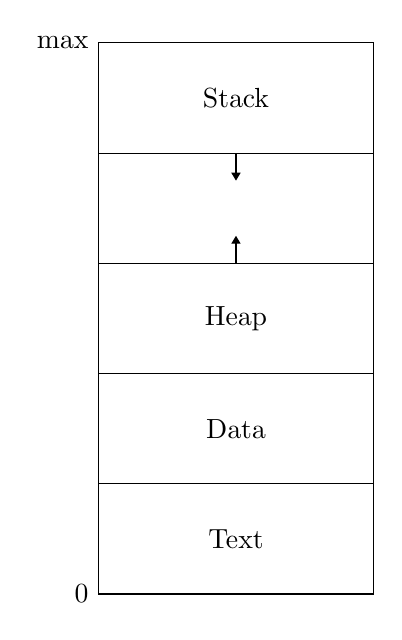
\begin{tikzpicture}[scale=0.7]
		\draw[-] (0,0) -- (0,10) -- (5,10) -- (5,0) -- (0,0);
		\draw[-] (0,2) -- (5,2);
		\draw[-] (0,4) -- (5,4);
		\draw[-] (0,6) -- (5,6);
		\draw[-] (0,8) -- (5,8);

		\draw (0,0) node[left] {0};
		\draw (0,10) node[left] {max};

		\draw (2.5,1) node {Text};
		\draw (2.5,3) node {Data};
		\draw (2.5,5) node {Heap};
		\draw (2.5,9) node {Stack};

		\draw[->] (2.5,8) -- (2.5,7.5);
		\draw[->] (2.5,6) -- (2.5,6.5);
	\end{tikzpicture}
	\caption{内存管理}
\end{figure}

\newpage
\chapter{封装}

\section{面向过程与面向对象}

\subsection{面向过程(Procedure Oriented)}

面向过程是一种以过程为中心的编程思想,以什么正在发生为主要目标进行编程,分析出解决问题所需要的步骤,然后用函数把这些步骤一步一步实现,使用的时候一个一个依次调用。\\

C语言就是一种面向过程的编程语言,但是面向过程的缺陷是数据和函数并不完全独立,使用两个不同的实体表示信息及其操作。\\

\subsection{面向对象(Object Oriented)}

面向对象是相对于面向过程来讲的,面向对象方法把相关的数据和方法组织为一个整体来看待,从更高的层次来进行系统建模,更贴近事物的自然运行模式。\\

在面向对象中,把构成问题的事物分解成各个对象,建立对象的目的不是为了完成一个步骤,而是为了描叙某个事物在整个解决问题的步骤中的行为。\\

Java、C++、Python等都是面向对象的编程语言,面向对象的优势在于只是用一个实体就能同时表示信息及其操作。\\

面向对象三大特性:

\begin{enumerate}
	\item 封装(encapsulation):数据和代码捆绑,避免外界干扰和不确定性访问。
	\item 继承(inheritance):让某种类型对象获得另一类型对象的属性和方法。
	\item 多态(polymorphism):同一事物表现出不同事物的能力。
\end{enumerate}

\newpage

\section{类与对象}

\subsection{类与对象}

类(class)表示同一类具有相同特征和行为的对象的集合,类定义了对象的属性和方法。\\

对象(object)是类的实例,对象拥有属性和方法。\\

类的设计需要使用关键字class,类名是一个标识符,遵循大驼峰命名法。类中可以包含属性和方法。其中,属性通过变量表示,又称实例变量;方法用于描述行为,又称实例方法。\\

通过关键字new进行对象的实例化,实例化对象会调用类中的构造函数完成。类是一种引用数据类型,对象的实例化在堆上开辟空间。\\

\mybox{类和对象}

\begin{lstlisting}[language=C++]
#include <iostream>
#include <string>

using namespace std;

class Person {
public:
    string name;
    int age;

    void eat() {
        cout << "吃饭" << endl;
    }

    void sleep() {
        cout << "睡觉" << endl;
    }
};

int main() {
    Person person;

    person.name = "小灰";
    person.age = 17;
    cout << "姓名:" << person.name << endl;
    cout << "年龄:" << person.age << endl;

    person.eat();
    person.sleep();
    return 0;
}
\end{lstlisting}

\begin{tcolorbox}
	\mybox{运行结果}
	\begin{verbatim}
姓名:小灰
年龄:17
吃饭
睡觉
	\end{verbatim}
\end{tcolorbox}

\newpage

\section{封装}

\subsection{封装(Encapsulation)}

封装是面向对象方法的重要原则,就是把对象的属性和方法结合为一个独立的整体,并尽可能隐藏对象的内部实现细节。\\

封装可以认为是一个保护屏障,防止该类的数据被外部类随意访问。要访问该类的数据,必须通过严格的接口控制。合适的封装可以让代码更容易理解和维护,也加强了程序的安全性。\\

实现封装的步骤:

\begin{enumerate}
	\item 修改属性的可见性来限制对属性的访问,一般限制为private。
	\item 对每个属性提供对外的公共方法访问,也就是提供一对setter / getter,用于对私有属性的访问。
\end{enumerate}

\vspace{0.5cm}

\subsection{访问权限}

属性和方法的访问权限一般分为3种:

\begin{enumerate}
	\item public:属性和方法在类的内部和外部都可以访问。
	\item private:属性和方法只能在类内访问。
	\item protected:属性和方法只能在类的内部和其派生类中访问。
\end{enumerate}

\vspace{0.5cm}

\subsection{this指针}

每一个对象都能通过this指针来访问自身的地址,this指针是所有成员方法的隐含参数,在成员方法内部可以用来指向调用对象。\\

在类中,属性的名字可以和局部变量的名字相同。此时,如果直接使用名字来访问,优先访问的是局部变量。因此,需要使用this指针来访问当前对象的属性。\\

当需要访问的属性与局部变量没有重名的时候,this可以省略。\\

\mybox{封装}

\begin{lstlisting}[language=C++]
#include <iostream>
#include <string>

using namespace std;

class Person {
public:
    void setName(string name) {
        this->name = name;
    }

    string getName() {
        return name;
    }

    void setAge(int age) {
        this->age = age;
    }

    int getAge() {
        return age;
    }

private:
    string name;
    int age;
};

int main() {
    Person person;

    person.setName("小灰");
    person.setAge(17);

    cout << "姓名:" << person.getName() << endl;
    cout << "年龄:" << person.getAge() << endl;
    return 0;
}
\end{lstlisting}

\begin{tcolorbox}
	\mybox{运行结果}
	\begin{verbatim}
姓名:小灰
年龄:17
	\end{verbatim}
\end{tcolorbox}

\newpage

\section{构造函数与析构函数}

\subsection{构造函数(Constructor)}

构造函数也是一个函数,用于实例化对象,在实例化对象的时候调用。一般情况下,使用构造函数是为了在实例化对象的同时,给一些属性进行初始化赋值。\\

构造函数和普通函数的区别:

\begin{enumerate}
	\item 构造函数的名字必须和类名一致。
	\item 构造函数没有返回值,返回值类型部分不写。
\end{enumerate}

如果一个类中没有构造函数,系统会自动提供一个public权限的无参构造函数以便实例化对象。如果一个类中已有构造函数,系统将不再提供任何默认的构造函数。\\

\mybox{构造函数}

\begin{lstlisting}[language=C++]
#include <iostream>
#include <string>

using namespace std;

class Person {
public:
    Person();
    Person(string name, int age);
    string toString();

private:
    string name;
    int age;
};

// 无参构造函数
Person::Person() {
    cout << "Person::Person()" << endl;
}

// 有参构造函数
Person::Person(string name, int age) {
    cout << "Person::Person(string, int)" << endl;
    this->name = name;
    this->age = age;
}

string Person::toString() {
    return "姓名:" + name + ",年龄:" + to_string(age);
}

int main() {
    Person p1;
    Person p2("小灰", 17);
    cout << p2.toString() << endl;
    return 0;
}
\end{lstlisting}

\begin{tcolorbox}
	\mybox{运行结果}
	\begin{verbatim}
Person::Person()
Person::Person(string, int)
姓名:小灰,年龄:17
	\end{verbatim}
\end{tcolorbox}

\vspace{0.5cm}

\subsection{初始化列表}

与其它函数不同,构造函数还可以有初始化列表。初始化列表以【:】开头,后跟一些列以逗号分割的初始化字段。\\

\mybox{初始化列表}

\begin{lstlisting}[language=C++]
#include <iostream>
#include <string>

using namespace std;

class Person {
public:
    Person(string name, int age);
    string toString();

private:
    string name;
    int age;
};

Person::Person(string name, int age) : name(name), age(age) {
    cout << "Person::Person(string, int)" << endl;
}

string Person::toString() {
    return "姓名:" + name + ",年龄:" + to_string(age);
}

int main() {
    Person person("小灰", 17);
    cout << person.toString() << endl;    
    return 0;
}
\end{lstlisting}

\begin{tcolorbox}
	\mybox{运行结果}
	\begin{verbatim}
Person::Person(string, int)
姓名:小灰,年龄:17
	\end{verbatim}
\end{tcolorbox}

有些时候初始化列表是不可或缺的,以下情况必须使用初始化列表:

\begin{enumerate}
	\item 常量成员:常量只能初始化不能赋值。

	\item 引用类型:引用必须在定义时初始化,且不能重新赋值。

	\item 没有默认构造函数的类类型:使用初始化列表可以不必调用默认构造函数来初始化,而是直接调用拷贝构造函数初始化。
\end{enumerate}

\vspace{0.5cm}

\subsection{析构函数(Destructor)}

析构函数与构造函数相反,当对象的生命周期结束时,会自动执行析构函数,用于做清理善后的事情。\\

析构函数的名称以【~】为前缀,后加类名称,它没有返回值和参数。\\

\mybox{析构函数}

\begin{lstlisting}[language=C++]
#include <iostream>
#include <string>

using namespace std;

class Person {
public:
    Person(string name, int age);
    ~Person();

private:
    string name;
    int age;
};

Person::Person(string name, int age) : name(name), age(age) {
    cout << "Person::Person(string, int)" << endl;
}

Person::~Person() {
    cout << "Person::~Person()" << endl;
}

int main() {
    Person p1("小灰", 17);
    Person *p2 = new Person("小白", 21);
    delete p2;
    return 0;
}
\end{lstlisting}

\begin{tcolorbox}
	\mybox{运行结果}
	\begin{verbatim}
Person::Person(string, int)
Person::Person(string, int)
Person::~Person()
Person::~Person()
	\end{verbatim}
\end{tcolorbox}

\vspace{0.5cm}

\subsection{拷贝构造函数(Copy Constructor)}

拷贝构造函数是构造函数的一种,它只有一个参数,参数类型为本类的引用。参数可以使const引用,也可以是非const引用,但是一般使用前者。\\

如果没有编写拷贝构造函数,编译器会自动生成一个默认的拷贝构造函数。\\

\mybox{拷贝构造函数}

\begin{lstlisting}[language=C++]
#include <iostream>
#include <string>

using namespace std;

class Person {
public:
    Person(const Person &p);
    Person(string name, int age);

private:
    string name;
    int age;
};

Person::Person(const Person &p) {
    cout << "Person::Person(const Person &)" << endl;
    this->name = p.name;
    this->age = p.age;
}

Person::Person(string name, int age) {
    cout << "Person::Person(string, int)" << endl;
    this->name = name;
    this->age = age;
}

int main() {
    Person p1("小灰", 17);
    Person p2(p1);
    Person p3 = p1;
    return 0;
}
\end{lstlisting}

\begin{tcolorbox}
	\mybox{运行结果}
	\begin{verbatim}
Person::Person(string, int)
Person::Person(const Person &)
Person::Person(const Person &)
	\end{verbatim}
\end{tcolorbox}

拷贝构造函数会在三种情况下被调用:

\begin{enumerate}
	\item 用一个对象去初始化同类的另一个对象。
	\item 函数参数是类的对象。
	\item 函数的返回值是类的对象。
\end{enumerate}

\vspace{0.5cm}

\subsection{浅拷贝 / 深拷贝}

当使用浅拷贝(shallow copy)时,仅仅是拷贝指针字面值,如果原来的对象调用析构函数释放掉指针所指向的数据,则会产生空悬指针(dangling pointer),因为所指向的内存空间已经被释放了。\\

\mybox{浅拷贝}

\begin{lstlisting}[language=C++]
#include <iostream>

using namespace std;

class User {
public:
    User();
    ~User();
    void printDataAddress();

private:
    int *data;
};

User::User() {
    this->data = new int;
}

User::~User() {
    delete data;
    data = nullptr;
}

void User::printDataAddress() {
    cout << data << endl;
}

int main() {
    User user1;
    user1.printDataAddress();
    User user2(user1);
    user2.printDataAddress();  
    return 0;
}
\end{lstlisting}

\begin{tcolorbox}
	\mybox{运行结果}
	\begin{verbatim}
0x26c2b90
0x26c2b90
	\end{verbatim}
\end{tcolorbox}

深拷贝(deep copy)可以解决浅拷贝出现的问题,通过定义一个拷贝构造函数,当被拷贝对象存在动态分配的存储空间时,需要先动态申请一块存储空间,然后逐字节拷贝内容。\\

\mybox{深拷贝}

\begin{lstlisting}[language=C++]
#include <iostream>

using namespace std;

class User {
public:
    User();
    User(const User& user);
    ~User();
    void printDataAddress();

private:
    int *data;
};

User::User() {
    this->data = new int;
}

User::User(const User& user) {
    this->data = new int;
    *(this->data) = *(user.data);
}

User::~User() {
    delete data;
    data = nullptr;
}

void User::printDataAddress() {
    cout << data << endl;
}

int main() {
    User user1;
    user1.printDataAddress();
    User user2(user1);
    user2.printDataAddress();  
    return 0;
}
\end{lstlisting}

\begin{tcolorbox}
	\mybox{运行结果}
	\begin{verbatim}
0x6b17b0
0x6b17d0
	\end{verbatim}
\end{tcolorbox}

\newpage

\section{静态成员}

\subsection{静态成员}

类的静态成员在编译时创建并初始化,在该类的任何对象建立之前就已经存在。静态成员不属于任何对象,并且在类中只有一份,为所有此类对象共享。\\

在静态成员函数的实现中不能直接引用类中的非静态成员,但可以引用类中的静态成员。如果静态成员函数中要引用非静态成员时,需要通过对象来引用。\\

\mybox{静态成员}

\begin{lstlisting}[language=C++]
#include <iostream>
#include <string>

using namespace std;

class User {
public:
    User(int id, string name) : id(id), name(name) {
        totalUsers++;
    }

    static int getTotalUsers() {
        return totalUsers;
    }

private:
    static int totalUsers;
    int id;
    string name;
};

int User::totalUsers = 0;       // 初始用户数量

int main() {
    cout << User::getTotalUsers() << endl;

    for(int i = 0; i < 10; i++) {
        User user(i, "User-" + to_string(i));
    }

    cout << User::getTotalUsers() << endl;
    return 0;
}
\end{lstlisting}

\begin{tcolorbox}
	\mybox{运行结果}
	\begin{verbatim}
0
10
	\end{verbatim}
\end{tcolorbox}

\newpage

\section{友元}

\subsection{友元函数}

封装使得类的数据对外隐藏,但是有些函数不是类的一部分,却又需要频繁访问类的数据成员,这时可以将这些函数定义为该类的友元函数。一个函数可以是多个类的友元函数,只需要在各个类中分别声明。除了友元函数,还有友元类。\\

友元(friend)的作用是提高程序的运行效率,减少了类型检查和安全性检查等需要的时间开销,但它破坏了类的封装性和隐藏性,使得非成员函数可以访问类的私有成员。\\

友元函数是可以直接访问类的私有成员的非成员函数。它是定义在类外的普通函数,它不属于任何类,但需要在类的定义中加以声明。

\vspace{-0.5cm}

\begin{lstlisting}[language=C++]
friend ret_type func_name([param_list]);
\end{lstlisting}

\vspace{0.5cm}

\mybox{友元函数}

\begin{lstlisting}[language=C++]
#include <iostream>
#include <cmath>

using namespace std;

class Coordinate {
public:
    Coordinate(double x, double y) : x(x), y(y) {};

    friend double distance(Coordinate &c1, Coordinate &c2);

private:
    double x;
    double y;
};

double distance(Coordinate &c1, Coordinate &c2) {
    double deltaX = c1.x - c2.x;
    double deltaY = c1.y - c2.y;
    return sqrt(deltaX * deltaX + deltaY * deltaY);
}

int main() {
    Coordinate c1(3, 5);
    Coordinate c2(4, 6);
    cout << distance(c1, c2) << endl;
    return 0;
}
\end{lstlisting}

\begin{tcolorbox}
	\mybox{运行结果}
	\begin{verbatim}
1.41421
	\end{verbatim}
\end{tcolorbox}

\vspace{0.5cm}

\subsection{友元类}

友元类的所有成员函数都是另一个类的友元函数,可以访问另一个类中的隐藏信息。当一个类想要存取另一个类的私有成员时,可以将该类声明为另一类的友元类。

\vspace{-0.5cm}

\begin{lstlisting}[language=C++]
friend class class_name;
\end{lstlisting}

友元有以下需要注意的地方:

\begin{enumerate}
	\item 友元关系不能被继承。
	\item 友元关系是单向的,不具有交换性。如果A是B的友元,B不一定是A的友元。
	\item 友元关系不具有传递性。如果A是B的友元,C是A的友元,那么C不一定是B的友元。
\end{enumerate}

\newpage

\section{运算符重载}

\subsection{运算符重载}

C++中预定义的运算符的操作对象只能是基本数据类型,但实际上对于许多用户自定义类型(例如类),也需要类似的运算操作。这时就必须在C++中重新定义这些运算符,赋予已有运算符新的功能,使它能够用于特定类型执行特定的操作。运算符重载的实质是函数重载,它提供了可扩展性。\\

运算符重载是通过创建运算符函数实现的,运算符函数定义了重载的运算符将要进行的操作。运算符函数的定义与其它函数的定义类似,惟一的区别是运算符函数的函数名是由关键字operator和要重载的运算符符号构成。

\vspace{-0.5cm}

\begin{lstlisting}[language=C++]
ret_type operator op([param_list]) {
    // code
}
\end{lstlisting}

运算符重载需要遵循以下规则:

\begin{enumerate}
	\item 除了【.】、【->】、【sizeof】、【?:】和【\#】,其它运算符都可以重载。

	\item 重载后的运算符不能改变优先级和结合性,也不能概念运算符的操作数个数及语法结构。

	\item 运算符重载是针对新类型数据对实际需要的改造,重载后的运算符应当与原有功能相类似。
\end{enumerate}

\vspace{0.5cm}

\subsection{二元运算符重载}

二元运算符需要两个操作数,例如【+】、【-】、【*】、【/】等。\\

\mybox{二元运算符重载}

\begin{lstlisting}[language=C++]
#include <iostream>
#include <string>

using namespace std;

class Complex {
public:
    Complex(int real, int imaginary);
    string getNumber();
    Complex operator+(const Complex& c);

private:
    int real;
    int imaginary;
};

Complex::Complex(int real = 0, int imaginary = 0)
    : real(real), imaginary(imaginary) {}

string Complex::getNumber() {
    return to_string(real) + "+" + to_string(imaginary) + "i";
}

Complex Complex::operator+(const Complex& c) {
    Complex complex;
    complex.real = this->real + c.real;
    complex.imaginary = this->imaginary + c.imaginary;
    return complex;
}

int main() {
    Complex c1(1, 2);
    Complex c2(8, 1);
    Complex result = c1 + c2;
    cout << result.getNumber() << endl;
    return 0;
}
\end{lstlisting}

\begin{tcolorbox}
	\mybox{运行结果}
	\begin{verbatim}
9+3i
	\end{verbatim}
\end{tcolorbox}

\vspace{0.5cm}

\subsection{一元运算符重载}

一元运算符只对一个操作数操作,例如【++】、【--】、【-】、【!】等。\\

\mybox{一元运算符重载}

\begin{lstlisting}[language=C++]
#include <iostream>
#include <string>
#include <iomanip>

using namespace std;

class Time {
public:
    Time(int hour, int minute, int second);
    void display();
    Time operator++();      // 前置++
    Time operator++(int);   // 后置++

private:
    int hour;
    int minute;
    int second;
};

Time::Time(int hour, int minute, int second) 
    : hour(hour), minute(minute), second(second) {}

void Time::display() {
    cout << setfill('0')
         << setw(2) << hour << ":"
         << setw(2) << minute << ":"
         << setw(2) << second << endl;
}

// 前置++
Time Time::operator++() {
    second++;
    if(second == 60) {
        second %= 60;
        minute++;
        if(minute == 60) {
            minute %= 60;
            hour++;
            if(hour == 24) {
                hour = 0;
            }
        }
    }
    return Time(hour, minute, second);
}

// 后置++
Time Time::operator++(int) {
    // 保存原始值
    Time time(hour, minute, second);
    second++;
    if(second == 60) {
        second %= 60;
        minute++;
        if(minute == 60) {
            minute %= 60;
            hour++;
            if(hour == 24) {
                hour = 0;
            }
        }
    }
    return time;    // 返回原始值
}

int main() {
    Time time(9, 21, 58);
    time.display();

    ++time;
    time.display();

    time++;
    time.display();
    return 0;
}
\end{lstlisting}

\begin{tcolorbox}
	\mybox{运行结果}
	\begin{verbatim}
09:21:58
09:21:59
09:22:00
	\end{verbatim}
\end{tcolorbox}

\vspace{0.5cm}

\subsection{输入输出运算符重载}

C++使用流提取运算符【>>】和流插入运算符【<<】进行输入输出,通过运算符重载可以对自定义对象进行输入输出操作。通过把输入输出运算符重载函数声明为类的友元,可以直接调用函数而无需创建对象。\\

\mybox{输入输出运算符重载}

\begin{lstlisting}[language=C++]
#include <iostream>
#include <string>
using namespace std;

class User {
public:
    User(int id, string name);
    friend ostream& operator<<(
        ostream& out,
        const User& user);
    friend istream& operator>>(istream& in, User& user);

private:
    int id;
    string name;
};

User::User(int id = 0, string name = "")
    : id(id), name(name) {}

ostream& operator<<(ostream& out, const User& user) {
    out << "ID: " << to_string(user.id) << ", "
        << "name: " << user.name;
    return out;
}

istream& operator>>(istream& in, User& user) {
    cout << "Enter user ID: ";
    in >> user.id;
    cout << "Enter user name: ";
    in >> user.name;
    return in;
}

int main() {
    User user;
    cin >> user;
    cout << user;
    return 0;
}
\end{lstlisting}

\begin{tcolorbox}
	\mybox{运行结果}
	\begin{verbatim}
Enter user ID: 1
Enter user name: Terry
ID: 1, name: Terry
	\end{verbatim}
\end{tcolorbox}

\newpage
\chapter{继承}

\section{继承}

\subsection{继承(Inheritance)}

继承是面向对象的三大特征之一,程序中的继承是类与类之间的特征和行为的一种赠予或获取。两个类之间的继承必须满足“is a”的关系。子类继承自父类,父类也称基类或超类,子类也称派生类。

\begin{figure}[H]
	\centering
	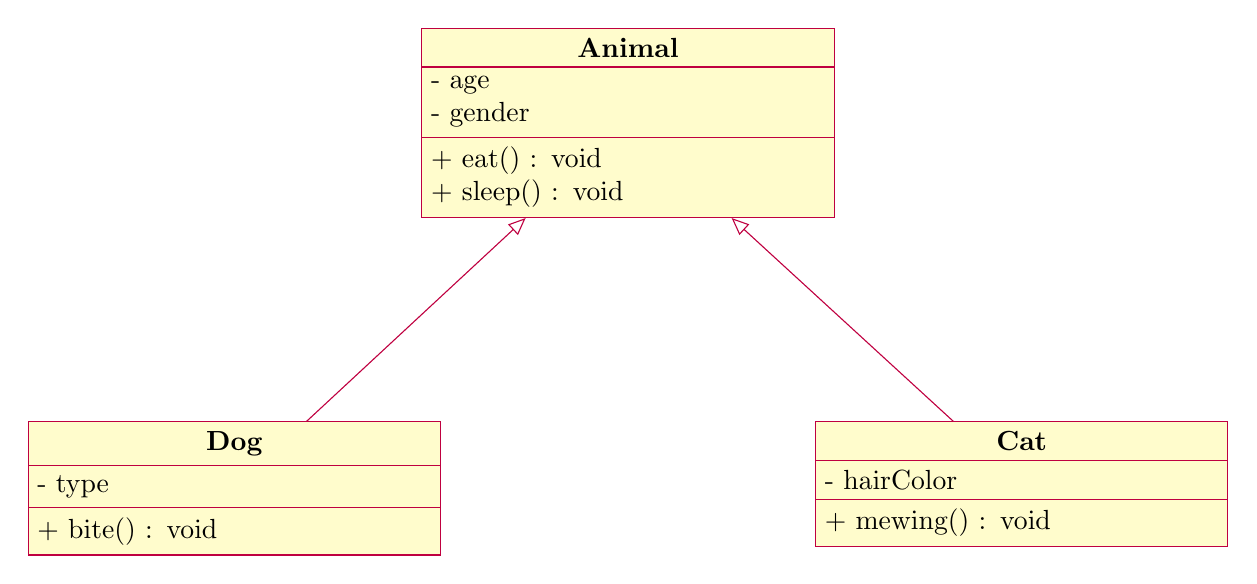
\begin{tikzpicture}
		\begin{class}{Animal}{0,0}
			\attribute{- age}
			\attribute{- gender}
			\operation{+ eat() : void}
			\operation{+ sleep() : void}
		\end{class}

		\begin{class}{Dog}{-5,-5}
			\inherit{Animal}
			\attribute{- type}
			\operation{+ bite() : void}
		\end{class}

		\begin{class}{Cat}{5,-5}
			\inherit{Animal}
			\attribute{- hairColor}
			\operation{+ mewing() : void}
		\end{class}
	\end{tikzpicture}
	\caption{继承}
\end{figure}

产生继承关系后,子类可以使用父类中的属性和方法,也可以定义子类独有的属性和方法。

\vspace{-0.5cm}

\begin{lstlisting}[language=Java]
class subclass : access_modifier superclass {
    // code
};
\end{lstlisting}

继承时通常使用public类型。当一个类public继承于父类时,父类的public成员也是子类的public成员,父类的protected成员也是子类的protected成员,父类的private成员不能被继承。\\

继承的好处是可以提高代码的复用性、提高代码的拓展性。\\

\mybox{继承}

\begin{lstlisting}[language=C++, title=animal.h]
#ifndef _ANIMAL_H_
#define _ANIMAL_H_

#include <string>

class Animal {
public:
    Animal(std::string name = "", int age = 0);
    void eat();

private:
    std::string name;
    int age;
};

#endif
\end{lstlisting}

\begin{lstlisting}[language=C++, title=animal.cpp]
#include "animal.h"
#include <iostream>

using namespace std;

Animal::Animal(string name, int age)
    : name(name), age(age) {}

void Animal::eat() {
    cout << "eating" << endl;
}
\end{lstlisting}

\begin{lstlisting}[language=C++, title=dog.h]
#ifndef _DOG_H
#define _DOG_H_

#include "animal.h"
#include <string>

class Dog : public Animal {
public:
    Dog(std::string name, int age, std::string type = "");
    void bite();
    
private:
    std::string type;
};

#endif
\end{lstlisting}

\begin{lstlisting}[language=C++, title=dog.cpp]
#include "dog.h"
#include <iostream>

using namespace std;

Dog::Dog(string name, int age, string type)
    : Animal(name, age), type(type) {}

void Dog::bite() {
    cout << "biting" << endl;
}
\end{lstlisting}

\begin{lstlisting}[language=C++, title=test\_dog.cpp]
#include <iostream>
#include "dog.h"

using namespace std;

int main() {
    Dog dog("狗子", 3, "哈士奇");
    dog.eat();
    dog.bite();
    return 0;
}
\end{lstlisting}

\begin{tcolorbox}
	\mybox{运行结果}
	\begin{verbatim}
eating
biting
	\end{verbatim}
\end{tcolorbox}

\newpage

\section{多继承}

\subsection{多继承}

C++支持多继承,即一个子类可以有两个或更多个父类。多继承时通过使用逗号将多个父类隔开,每个父类都可以用不同访问限定符修饰。\\

当多个父类中有同名的成员时,就会产生命名冲突,因此这时就需要在成员前加上类名和域限定符【::】消除二义性。\\

\mybox{多继承}

\begin{lstlisting}[language=C++, title=date.h]
#ifndef _DATE_H_
#define _DATE_H_

#include <string>

class Date {
public:
    Date(int year = 1970, int month = 1, int day = 1);
    std::string getDate();

private:
    int year;
    int month;
    int day;
};

#endif
\end{lstlisting}

\begin{lstlisting}[language=C++, title=date.cpp]
#include "date.h"

using namespace std;

Date::Date(int year, int month, int day)
    : year(year), month(month), day(day) {}

string Date::getDate() {
    char format[128];
    snprintf(format, sizeof(format), 
            "%04d/%02d/%02d", year, month, day);
    string dateStr(format);
    return dateStr;
}
\end{lstlisting}

\begin{lstlisting}[language=C++, title=time.h]
#ifndef _TIME_H_
#define _TIME_H_

#include <string>

class Time {
public:
    Time(int hour = 0, int minute = 0, int second = 0);
    std::string getTime();

private:
    int hour;
    int minute;
    int second;
};

#endif
\end{lstlisting}

\begin{lstlisting}[language=C++, title=time.cpp]
#include "time.h"

using namespace std;

Time::Time(int hour, int minute, int second)
    : hour(hour), minute(minute), second(second) {}

string Time::getTime() {
    char format[128];
    snprintf(format, sizeof(format), 
            "%02d:%02d:%02d", hour, minute, second);
    string timeStr(format);
    return timeStr;
}
\end{lstlisting}

\begin{lstlisting}[language=C++, title=date\_time.h]
#ifndef _DATE_TIME_H_
#define _DATE_TIME_H_

#include "date.h"
#include "time.h"
#include <string>

class DateTime : public Date, public Time {
public:
    DateTime(int year = 1970, int month = 1, int day = 1,
             int hour = 0, int minute = 0, int second = 0);
    std::string getDateTime();

private:
    int year;
    int month;
    int day;
    int hour;
    int minute;
    int second;
};

#endif
\end{lstlisting}

\begin{lstlisting}[language=C++, title=date\_time.cpp]
#include "date_time.h"

using namespace std;

DateTime::DateTime(int year, int month, int day,
         int hour, int minute, int second)
  : Date(year, month, day),
    Time(hour, minute, second) {}

string DateTime::getDateTime() {
    return getDate() + " " + getTime();
}
\end{lstlisting}

\begin{lstlisting}[language=C++, title=test\_date\_time.cpp]
#include <iostream>
#include "date_time.h"

using namespace std;

int main() {
    DateTime dt1;
    cout << dt1.getDateTime() << endl;
    DateTime dt2(2021, 8, 31, 13, 50, 23);
    cout << dt2.getDateTime() << endl;
    return 0;
}
\end{lstlisting}

\begin{tcolorbox}
	\mybox{运行结果}
	\begin{verbatim}
1970/01/01 00:00:00
2021/08/31 13:50:23
	\end{verbatim}
\end{tcolorbox}

\newpage

\section{向上转型与向下转型}

\subsection{向上转型 / 向下转型}

对象由子类类型转型为父类类型,即是向上转型。向上转型是一种隐式转换,一定会转型成功。向上转型后的对象,只能访问父类中定义的成员。\\

由父类类型转型转型为子类类型,即是向下转型。向下转型是不安全的,可能会导致数据的丢失,原因是父类的指针或引用中可能不包含子类成员的内存。\\

\mybox{向上转型}

\begin{lstlisting}[language=C++, title=animal.h]
#ifndef _ANIMAL_H_
#define _ANIMAL_H_

#include <string>

class Animal {
public:
    Animal(std::string name = "");
    std::string getName();

private:
    std::string name;
};

#endif
\end{lstlisting}

\begin{lstlisting}[language=C++, title=animal.cpp]
#include "animal.h"

using namespace std;

Animal::Animal(string name) : name(name) {}

string Animal::getName() {
    return name;
}
\end{lstlisting}

\begin{lstlisting}[language=C++, title=dog.h]
#ifndef _DOG_H_
#define _DOG_H_

#include "animal.h"
#include <string>

class Dog : public Animal {
public:
    Dog(std::string name, std::string type = "");
    std::string getType();

private:
    std::string type;
};

#endif
\end{lstlisting}

\begin{lstlisting}[language=C++, title=dog.cpp]
#include "dog.h"

using namespace std;

Dog::Dog(string name, string type) 
    : Animal(name), type(type) {}

string Dog::getType() {
    return type;
}
\end{lstlisting}

\begin{lstlisting}[language=C++, title=test\_dog.cpp]
#include <iostream>
#include "animal.h"
#include "dog.h"

using namespace std;

int main() {
    Dog dog("狗子", "哈士奇");
    cout << "dog: " << dog.getName()
         << ", " << dog.getType() << endl; 

    Animal animal = (Animal)dog;
    cout << "animal: " << animal.getName() << endl;
    return 0;
}
\end{lstlisting}

\begin{tcolorbox}
	\mybox{运行结果}
	\begin{verbatim}
dog: 狗子, 哈士奇
animal: 狗子
    \end{verbatim}
\end{tcolorbox}

\newpage
\chapter{多态}

\section{多态}

\subsection{多态(Polymorphism)}

多态是同一个行为具有多个不同表现形式或形态的能力。

\begin{figure}[H]
	\centering
	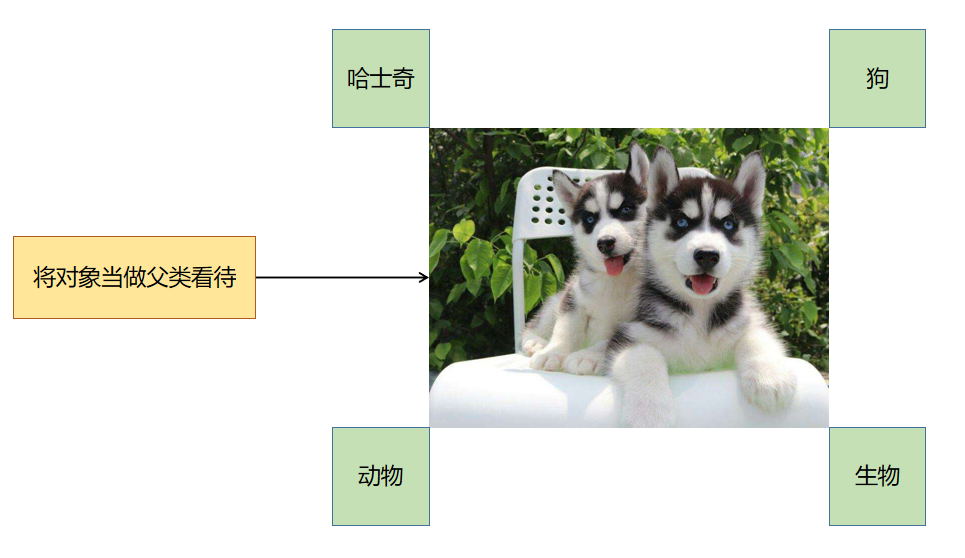
\includegraphics[scale=0.7]{img/C4/4-1/1.png}
	\caption{多态}
\end{figure}

\begin{figure}[H]
	\centering
	\begin{tikzpicture}[]
		\draw (0,0) node {Animal animal = new Dog();};

		\draw (-3,-2) rectangle (-1,-1);
		\draw (1,-2) rectangle (3,-1);
		\draw (-2,-1.5) node {父类引用};
		\draw (2,-1.5) node {子类对象};

		\draw[->] (-2,-1) -- (-1.5,-0.3);
		\draw[->] (2,-1) -- (1.5,-0.3);
	\end{tikzpicture}
	\caption{父类引用指向子类对象}
\end{figure}

通过父类引用指向子类对象,从而产生多种形态。父类引用仅能访问父类所声明的属性和方法,不能访问子类独有的属性和方法。 \\

在一对有继承关系的类中都有一个方法,其方法名、参数列表、返回值均相同,通过调用方法实现不同类对象完成不同的事件。 \\

构成多态需要满足三个条件:

\begin{enumerate}
	\item 必须存在继承关系。
	\item 继承关系中必须有同名的虚函数。
	\item 存在基类类型的指针或引用,通过该指针或引用调用虚函数。
\end{enumerate}

\newpage

\section{虚函数}

\subsection{虚函数}


\chapter{异常}

\section{异常}

\subsection{异常(Exception)}

异常就是程序在运行过程中出现的非正常的情况。异常本身是一个类,产生异常就是创建异常对象并抛出一个异常对象。Java处理异常的方法是中断处理。 \\

C++异常处理涉及到三个关键字:

\begin{enumerate}
	\item throw:当问题出现时,程序会抛出一个异常。
	\item try:放置可能抛出异常的代码。
	\item catch:捕获并处理异常。
\end{enumerate}

\begin{figure}[H]
	\centering
	
\includegraphics{img/C5/5-1/1.png}
\end{figure}

\mybox{除以0}

\begin{lstlisting}[language=C++]
#include <iostream>

using namespace std;

int divide(int num1, int num2) {
    if(num2 == 0) {
        throw "division by zero";
    }
    return num1 / num2;
}

int main() {
    try {
        int result = divide(5, 0);
        cout << result << endl;
    } catch(const char *msg) {
        cerr << msg << endl;
    }

    return 0;
}
\end{lstlisting}

\begin{tcolorbox}
	\mybox{运行结果}
	\begin{verbatim}
division by zero
	\end{verbatim}
\end{tcolorbox}

普通的异常会导致程序无法完成编译,这样的异常被称为非运行时异常(non-runtime exception),但是由于异常是发生在编译时期的,因此常常称为编译时异常。在运行中如果遇到了异常,会导致程序执行的强制停止,这样的异常被称为运行时异常。

\newpage

\section{异常类}

C++提供了一系列标准的异常,定义在<exception>中。

\begin{table}[H]
	\centering
	\setlength{\tabcolsep}{5mm}{
		\begin{tabular}{|c|l|}
			\hline
			\textbf{异常}          & \textbf{描述}         \\
			\hline
			std::exception         & 所有标准C++异常的父类 \\
			\hline
			std::bad\_alloc        & 通过new抛出           \\
			\hline
			std::bad\_cast         & 通过dynamic\_cast抛出 \\
			\hline
			std::bad\_exception    & 处理无法预期的异常    \\
			\hline
			std::bad\_typeid       & 通过typeid抛出        \\
			\hline
			std::logic\_error      & 逻辑错误              \\
			\hline
			std::domain\_error     & 使用了无效的定义域    \\
			\hline
			std::invalid\_argument & 使用了无效的参数      \\
			\hline
			std::length\_error     & 创建过长的std::string \\
			\hline
			std::out\_of\_range    & 访问定义外的元素      \\
			\hline
			std::runtime\_error    & 运行时错误            \\
			\hline
			std::overflow\_error   & 发生上溢              \\
			\hline
			std::underflow\_error  & 发生下溢              \\
			\hline
			std::range\_error      & 存储超出范围的值      \\
			\hline
		\end{tabular}
	}
	\caption{异常类}
\end{table}

what()是异常类提供的一个公共方法,它已被所有子异常类重载。 \\

\mybox{bad\_alloc}

\begin{lstlisting}[language=C++]
#include <iostream>
#include <exception>

using namespace std;

int main() {
    try {
        char *p = new char[0xfffffffff];
        delete p;
    } catch(bad_alloc &e) {
        cerr << e.what() << endl;
    }
    return 0;
}
\end{lstlisting}

\begin{tcolorbox}
	\mybox{运行结果}
	\begin{verbatim}
std::bad_alloc
	\end{verbatim}
\end{tcolorbox}

\newpage

\section{自定义异常}

\subsection{自定义异常}

系统中提供了很多的异常类型,但是异常类型提供地再多,也无法满足所有的需求。当需要的异常类型系统没有提供的时候,此时就需要自定义异常了。通过继承和重载exception类可以定义新的异常。 \\

\mybox{自定义异常}

\begin{lstlisting}[language=C++]
#include <iostream>
#include <string>
#include <exception>

using namespace std;

class AgeException : public exception {
public:
    AgeException(string msg) : msg(msg) {}

    virtual const char* what() const noexcept override {
        return msg.c_str();
    }

private:
    string msg;
};

int main() {
    try {
        int age;
        cout << "Enter age: ";
        cin >> age;
        if(age < 0 || age > 130) {
            throw AgeException("invalid age");
        }
    } catch(AgeException& e) {
        cout << e.what() << endl;
    }

    return 0;
}
\end{lstlisting}

\begin{tcolorbox}
	\mybox{运行结果}
	\begin{verbatim}
Enter age: -1
invalid age
	\end{verbatim}
\end{tcolorbox}

\newpage
\chapter{I/O库}

\section{标准I/O}

\subsection{标准I/O}

C++不直接处理输入输出,而是通过标准库中的一组类来处理I/O。输入流istream提供输入,输出流ostream提供输出。\\

标准输入输出有以下特点:

\begin{enumerate}
	\item cin是istream的对象,从标准输入读取数据。
	\item cout是ostream的对象,向标准输出写数据。
	\item cerr是ostream的对象,用于输出错误信息,写到标准错误。
	\item 【>>】运算符从istream对象读取输入。
	\item 【<<】运算符从ostream对象写输出。
	\item getline()从给定的`istream`读取一行数据,存入string对象。
\end{enumerate}

\vspace{0.5cm}

\subsection{I/O格式化}

每个iostream对象维护一个格式状态来控制I/O的细节,如进制、精度、宽度等。操纵符改变流的格式状态时,通常改变后的状态对所有后续I/O都生效。\\

标准库定义了一组操纵符用来修改流的格式状态:

\begin{table}[H]
	\centering
	\setlength{\tabcolsep}{5mm}{
		\begin{tabular}{|c|l|}
			\hline
			\textbf{操纵符} & \textbf{功能}                           \\
			\hline
			boolalpha       & 将true和false输出为字符串               \\
			\hline
			noboolalpha     & 将true和false输出为1和0                 \\
			\hline
			showbase        & 对整型值输出表示进制的前缀              \\
			\hline
			noshowbase      & 不生成表示进制的前缀                    \\
			\hline
			showpoint       & 浮点数总是显示小数点                    \\
			\hline
			noshowpoint     & 只有浮点数包含小数部分才显示小数点      \\
			\hline
			showpos         & 非负数显示【+】                         \\
			\hline
			noshowpos       & 非负数不显示【+】                       \\
			\hline
			uppercase       & 在十六进制中打印0X,在科学计数法中打印E \\
			\hline
			nouppercase     & 在十六进制中打印0x,在科学计数法中打印e \\
			\hline
			dec             & 整型显示为十进制                        \\
			\hline
			hex             & 整型显示为十六进制                      \\
			\hline
			oct             & 整型显示为八进制                        \\
			\hline
			left            & 在值的左侧添加填充字符                  \\
			\hline
			right           & 在值的右侧添加填充字符                  \\
			\hline
			internal        & 在符号和值之间添加填充字符              \\
			\hline
			fixed           & 浮点数显示为定点十进制                  \\
			\hline
			scientific      & 浮点数显示为科学计数法                  \\
			\hline
			unitbuf         & 每次输出操作后刷新缓冲区                \\
			\hline
			nounitbuf       & 恢复正常的缓冲区刷新方式                \\
			\hline
			skipws          & 输入运算符跳过空白符                    \\
			\hline
			noskipws        & 输入运算符不跳过空白符                  \\
			\hline
			flush           & 刷新ostream缓冲区                       \\
			\hline
			ends            & 插入空字符,然后刷新ostream缓冲区       \\
			\hline
			endl            & 插入换行符,然后刷新ostream缓冲区       \\
			\hline
			setfill(ch)     & 用ch填充空白                            \\
			\hline
			setprecision(n) & 将浮点精度设置为n                       \\
			\hline
			setw(n)         & 读或写值的宽度为n个字符                 \\
			\hline
			setbase(n)      & 将整数输出为n进制                       \\
			\hline
		\end{tabular}
	}
	\caption{操纵符}
\end{table}

\mybox{格式化输出}

\begin{lstlisting}[language=C++]
#include <iostream>
#include <cmath>
#include <iomanip>

using namespace std;

int main() {
    cout << "布尔:";
    cout << boolalpha << true << " " << false << endl;
    cout << "------------------------------" << endl;
    
    cout << "十进制:";
    cout << dec << 20 << " " << 1024 << endl;
    
    cout << "十六进制:";
    cout << showbase << hex 
        << 20 << " "<< 1024
        << noshowbase << endl;
    
    cout << "八进制:";
    cout << oct << 20 << " " << 1024 << dec << endl;
    cout << "------------------------------" << endl;
    
    cout << "科学计数法:";
    cout << scientific
        << 100 * sqrt(2)
        << defaultfloat << endl;
    cout << "------------------------------" << endl;
    
    cout << "默认输出浮点数:";
    cout << 10.0 << endl;
    
    cout << "浮点数打印小数点:";
    cout << showpoint << 10.0 << noshowpoint << endl;
    cout << "------------------------------" << endl;
    
    cout << "精度:";
    cout << setprecision(3) << fixed << sqrt(2) << endl;
    cout << "------------------------------" << endl;
    
    cout << "宽度填充:";
    cout << setfill('0') << setw(4) << 2021 << "/"
         << setw(2) << 9 << "/"
         << setw(2) << 2 << endl;
    return 0;
}
\end{lstlisting}

\begin{tcolorbox}
	\mybox{运行结果}
	\begin{verbatim}
布尔:true false
------------------------------
十进制:20 1024
十六进制:0x14 0x400
八进制:24 2000
------------------------------
科学计数法:1.414214e+02
------------------------------
默认输出浮点数:10
浮点数打印小数点:10.0000
------------------------------
精度:1.414
------------------------------
宽度填充:2021/09/02
	\end{verbatim}
\end{tcolorbox}

\newpage

\section{文件I/O}

\subsection{文件I/O}

程序不仅要从控制台进行I/O,还需要读写文件和字符串。\\

标准库的I/O类型在3个头文件中:

\begin{enumerate}
	\item <iostream>定义了读写流的基本类型。
	\item <fstream>定义了读写文件的类型。
	\item <sstream>定义了读写string对象的类型。
\end{enumerate}

<fstream>中定义了3个I/O类来读写文件:

\begin{enumerate}
	\item ifstream从给定文件读数据。
	\item ofstream向给定文件写数据。
	\item fstream可读写文件。
\end{enumerate}

\vspace{0.5cm}

\subsection{文件打开模式}

每个流都有一个关联的文件模式,在打开文件时可以指定文件模式。

\begin{table}[H]
	\centering
	\setlength{\tabcolsep}{5mm}{
		\begin{tabular}{|c|l|}
			\hline
			\textbf{打开模式} & \textbf{作用}                                   \\
			\hline
			ios::in           & 以读方式打开                                    \\
			\hline
			ios::out          & 以写方式打开                                    \\
			\hline
			ios::app          & 以追加方式打开                                  \\
			\hline
			ios::ate          & 打开文件定位到文件末尾                          \\
			\hline
			ios::trunc        & 如果文件存在,其内容将被截断,即把文件长度设为0 \\
			\hline
		\end{tabular}
	}
	\caption{文件打开模式}
\end{table}

\mybox{文件I/O}

\begin{lstlisting}[language=C++]
#include <iostream>
#include <fstream>

using namespace std;

int main() {
    string name;
    int id;
    cout << "Enter name: ";
    cin >> name;
    cout << "Enter id: ";
    cin >> id;
    
    ofstream out("info.txt");
    out << name << " " << id << endl;
    out.close();
    
    ifstream in("info.txt");
    in >> name >> id;
    in.close();
    
    cout << "name = " << name << ", id = " << id << endl;
    return 0;
}
\end{lstlisting}

\begin{tcolorbox}
	\mybox{运行结果}
	\begin{verbatim}
Enter name: Terry
Enter id: 979489
name = Terry, id = 979489
	\end{verbatim}
\end{tcolorbox}

\newpage

\section{string流}

\subsection{string流}

<sstream>定义了3个类来支持内存IO:

\begin{enumerate}
	\item istringstream从string读数据。
	\item ostringstream向string写数据。
	\item stringstream可读写string。
\end{enumerate}

\mybox{string流}

\begin{lstlisting}[language=C++]
#include <iostream>
#include <sstream>
#include <string>

using namespace std;

int main() {
    string line;
    cout << "convert a string to Python list format: ";
    getline(cin, line);

    ostringstream out;
    istringstream in(line);
    string token;

    out << "[";
    while(in >> token) {
        out << token << ", ";
    }
    out << "\b\b]";
    cout << out.str() << endl;
    return 0;
}
\end{lstlisting}

\begin{tcolorbox}
	\mybox{运行结果}
	\begin{verbatim}
convert a string to Python list format: This is a test
[This, is, a, test]
	\end{verbatim}
\end{tcolorbox}

\newpage
\chapter{STL标准模板库}

\section{模板}

\subsection{泛型编程(Generic Programming)}

面向对象编程(OOP)和泛型编程(GP)都能处理在编写程序时类型未知的情况,OOP能处理运行时获取类型的情况,GP能处理编译期可获取类型的情况。 \\

模板是泛型编程的基础,泛型编程就是以一种独立于任何特定类型的方式编写代码。C++标准库的容器、迭代器、算法都是泛型编程的例子。

\subsection{函数模板}

通过定义一个通用的函数模板可以处理参数为多种类型的情形,而不是为每个类型都定义一个重载。模板定义使用template关键字,后跟模板参数列表。模板参数表示函数或类定义中用到的类型,使用模板时需要隐式或显式提供模板实参,将其绑定到模板参数。 \\

\mybox{函数模板}

\begin{lstlisting}[language=C++]
#include <iostream>
#include <string>

using namespace std;

template <typename T>
inline T getMax(const T& val1, const T& val2) {
    return val1 > val2 ? val1 : val2;
}

int main() {
    int iVal1 = 28;
    int iVal2 = 92;
    cout << getMax(iVal1, iVal2) << endl;

    double dVal1 = 3.14;
    double dVal2 = 3.71;
    cout << getMax(dVal1, dVal2) << endl;

    string sVal1 = "hello";
    string sVal2 = "world";
    cout << getMax(sVal1, sVal2) << endl;
    return 0;
}
\end{lstlisting}

\begin{tcolorbox}
	\mybox{运行结果}
	\begin{verbatim}
92
3.71
world
	\end{verbatim}
\end{tcolorbox}

函数模板仅仅是函数的规范,本身并不会占用内存。当编译器遇到对模板函数的调用时,才会在内存中创建该函数的实例。

\subsection{类模板}

类模板用来生成类的蓝图,与函数模板不同的是,类模板在实例化时编译器无法为类模板推导模板参数类型,而是必须在模板名后用【<>】提供实参。根据显式提供的模板实参列表,编译器使用这些模板参数来实例化特定的类。 \\

编译器从类模板实例化一个类时,会重写模板,将模板参数的每个实例替换为给定的模板实参。因此类模板的每个实例都是独立的类,使用不同模板实参实例化出的类之间没有关联,也没有特殊的访问权限。 \\

\mybox{类模板}

\begin{lstlisting}[language=C++]
#include <iostream>
#include <sstream>
#include <algorithm>

using namespace std;

template<class T>
class SortedArray {
public:
    SortedArray(int capacity = 1);
    SortedArray(T *arr, int capacity);
    ~SortedArray();

    string data();
    void add(T val);
    void remove(T val);

private:
    T *arr;
    int len;
    int capacity;
    void resize(int size);
};

template<class T>
SortedArray<T>::SortedArray(int capacity) {
    this->len = 0;
    this->capacity = capacity;
    this->arr = new T[capacity];
}

template<class T>
SortedArray<T>::SortedArray(T *arr, int len) {
    this->len = len;
    this->capacity = len;
    this->arr = new T[len];
    for(int i = 0; i < len; i++) {
        this->arr[i] = arr[i];
    }
}

template<class T>
SortedArray<T>::~SortedArray() {
    delete arr;
}

template<class T>
string SortedArray<T>::data() {
    if(len == 0) {
        return "[]";
    }

    sort(this->arr, this->arr + len);
    ostringstream out;
    out << "[";
    for(int i = 0; i < len; i++) {
        out << arr[i] << ", ";
    }
    out << "\b\b]";
    return out.str();
}

template<class T>
void SortedArray<T>::resize(int size) {
    T *temp = new T[size];
    for(int i = 0; i < len; i++) {
        temp[i] = arr[i];
    }
    delete arr;
    arr = temp;
}

template<class T>
void SortedArray<T>::add(T val) {
    if(len == capacity) {
        capacity *= 2;
        resize(capacity);
    }
    arr[len++] = val;
}

template<class T>
void SortedArray<T>::remove(T val) {
    for(int i = 0; i < len; i++) {
        if(arr[i] == val) {
            arr[i] = arr[len-1];
            len--;
            if(len <= capacity / 2) {
                capacity /= 2;
                resize(capacity);
            }
            break;
        }
    }
}

int main() {
    int arr[] = {7, 7, 3, 9, 7, 1, 3};
    int n = sizeof(arr) / sizeof(arr[0]);

    SortedArray<int> sortedArray(arr, n);
    cout << sortedArray.data() << endl;

    sortedArray.add(28);
    sortedArray.add(12);
    cout << sortedArray.data() << endl;

    sortedArray.remove(7);
    sortedArray.remove(9);
    cout << sortedArray.data() << endl;

    return 0;
}
\end{lstlisting}

\begin{tcolorbox}
	\mybox{运行结果}
	\begin{verbatim}
[1, 3, 3, 7, 7, 7, 9] 
[1, 3, 3, 7, 7, 7, 9, 12, 28]
[1, 3, 3, 7, 7, 12, 28]
	\end{verbatim}
\end{tcolorbox}

\newpage

\section{容器}

\subsection{容器(Container)}

容器是特定类型对象的集合,容器分为顺序容器和关联容器:

\begin{itemize}
	\item 顺序容器:元素的顺序与其加入容器的位置对应。
	\item 关联容器:元素的顺序由其关联的关键字决定,关联容器分为有序关联容器和无序关联容器。
\end{itemize}

所有容器类共享公有接口,不同容器按不同方式扩展。 \\

C++新标准容器的性能比旧版本快很多,其性能与最精心优化过的同类数据结构一样好。现代C++程序应该使用标准库容器,而不是更原始的数据结构。

\subsection{顺序容器}

每个容器都定义于一个头文件中,文件名与容器名相同。容器都定义为模板类,顺序容器几乎可以保存任意类型的元素,还可以在容器中保存容器。 \\

顺序容器包括array、vector、string、deque、list和forward\_list。

\begin{table}[H]
	\centering
	\setlength{\tabcolsep}{5mm}{
		\begin{tabular}{|c|l|}
			\hline
			\textbf{容器} & \textbf{描述}                                      \\
			\hline
			array         & 固定大小数组,支持快速随机访问,不能增删元素       \\
			\hline
			vector        & 可变大小数组,支持快速随机访问,非尾部位置增删较慢 \\
			\hline
			string        & 专门用于保存字符,随机访问快,在尾部增删速度快     \\
			\hline
			deque         & 双端队列,支持快速随机访问,在头尾位置增删速度很快 \\
			\hline
			list          & 双向链表,支持双向顺序访问,在任何位置增删都很快   \\
			\hline
			forward\_list & 单向链表,只支持单向顺序访问,在任何位置增删都很快 \\
			\hline
		\end{tabular}
	}
	\caption{顺序容器}
\end{table}

array和内置数组一样大小固定,但操作更安全。除固定大小的array外,其它容器都提供高效灵活的内存管理,可以添加、删除、扩展和收缩容器的大小。 \\

vector和string将元素存储在连续空间中,故通过下标的随机访问很快。在尾部添加元素很快,但中间和头部插入或删除很慢。添加元素可能造成空间的重新分配和元素拷贝。 \\

deque支持快速随机访问,在两端插入或删除很快,但在中间插入或删除元素很慢。 \\

list和forward\_list的设计目的是让任何位置的插入或删除都快速高效且不需重新分配内存,但是不支持随机访问,为访问一个元素需要遍历整个链表。

\subsection{迭代器(Iterator)}

迭代器比下标访问更通用,所有标准库容器都支持迭代器,但只有几种支持下标。迭代器提供了对容器对象的间接访问,类似于指针。begin()返回指向首元素的迭代器,end()返回指向尾元素下一位置(尾后)的迭代器。如果容器为空,则begin()和end()返回的都是尾后迭代器。 \\

任何可能改变容器容量的操作都会使容器的迭代器失效。

\begin{table}[H]
	\centering
	\setlength{\tabcolsep}{5mm}{
		\begin{tabular}{|l|l|}
			\hline
			\textbf{容器}            & \textbf{描述}                  \\
			\hline
			iterator                 & 容器的迭代器                   \\
			\hline
			begin()                  & 返回指向首元素的迭代器         \\
			\hline
			end()                    & 返回尾后迭代器                 \\
			\hline
			const\_iterator          & 只读迭代器                     \\
			\hline
			cbegin()                 & 返回指向首元素的只读迭代器     \\
			\hline
			cend()                   & 返回尾后只读迭代器             \\
			\hline
			reverse\_iterator        & 按逆序寻址元素的迭代器         \\
			\hline
			rbegin()                 & 返回指向尾元素的逆序迭代器     \\
			\hline
			rend()                   & 返回首前逆序迭代器             \\
			\hline
			const\_reverse\_iterator & 只读逆序迭代器                 \\
			\hline
			crbegin()                & 返回指向尾元素的只读逆序迭代器 \\
			\hline
			crend()                  & 返回首前只读逆序迭代器         \\
			\hline
		\end{tabular}
	}
	\caption{迭代器}
\end{table}

迭代器可以进行算术运算,将迭代器与整数相加减可以得到向前或向后若干位置的迭代器。使用关系运算符【<】、【<=】、【>】、【>=】和【==】可以对迭代器所指位置比较大小。将两个迭代器相减,结果是两个迭代器的距离。 \\

\mybox{迭代器}

\begin{lstlisting}[language=C++]
#include <iostream>
#include <string>

using namespace std;

int main() {
    string s = "hello world";

    string::iterator iter = s.begin();
    cout << "[";
    while(iter != s.end()) {
        cout << *iter << ", ";
        iter++;
    }
    cout << "\b\b]" << endl;

    return 0;
}
\end{lstlisting}

\begin{tcolorbox}
	\mybox{运行结果}
	\begin{verbatim}
[h, e, l, l, o,  , w, o, r, l, d]
	\end{verbatim}
\end{tcolorbox}

\newpage

\section{STL数组}

\subsection{array}

array容器是C++11标准中新增的序列容器,它在普通数组的基础上,添加了一些成员函数和全局函数。在使用上,它比普通数组更安全,且效率并没有因此变差。和其它容器不同,array的大小是固定的,无法动态的扩展或收缩。与内置数组不同的是,array允许做整个容器的拷贝和赋值,要求两个array大小和元素类型都一样。 \\

array以类模板的形式定义在<array>头文件,array具有固定大小,其大小也是类型的一部分,定义时模板参数包含元素类型和大小。

\begin{table}[H]
	\centering
	\setlength{\tabcolsep}{5mm}{
		\begin{tabular}{|c|l|}
			\hline
			\textbf{成员函数} & \textbf{功能}                            \\
			\hline
			size()            & 返回容器中当前元素的数量                 \\
			\hline
			max\_size()       & 返回容器可容纳元素的最大数量             \\
			\hline
			empty()           & 判断容器是否为空                         \\
			\hline
			at(n)             & 返回容器中第n个元素的引用                \\
			\hline
			front()           & 返回容器中第一个元素的直接引用           \\
			\hline
			back()            & 返回容器中最后一个元素的直接应用         \\
			\hline
			data()            & 返回一个指向容器首个元素的指针           \\
			\hline
			fill(val)         & 将val赋值给容器中的每个元素              \\
			\hline
			arr1.swap(arr2)   & 交换相同长度和类型的arr1和arr2中所有元素 \\
			\hline
		\end{tabular}
	}
	\caption{array成员函数}
\end{table}

\mybox{array}

\begin{lstlisting}[language=C++]
#include <iostream>
#include <array>

using namespace std;

int main() {
    array<int, 10> arr = {0, 1, 2, 3, 4, 5, 6, 7, 8, 9};
    cout << "size = " << arr.size() << endl;
    array<int, 10>::iterator begin = arr.begin();
    array<int, 10>::iterator end = arr.end();
    while(begin != end) {
        cout << *begin << " ";
        begin++;
    }
    cout << endl;
    return 0;
}
\end{lstlisting}

\begin{tcolorbox}
	\mybox{运行结果}
	\begin{verbatim}
size = 10
0 1 2 3 4 5 6 7 8 9
	\end{verbatim}
\end{tcolorbox}

\subsection{vector}

vector表示对象的集合,由于vector容纳其它的对象,所以是一种容器。使用vector需要包含头文件<vector>。vector是一个类模板,模板可以看作编译器生成类或函数的一份说明。 \\

vector的初始化包括直接初始化、拷贝初始化和列表初始化。

\begin{table}[H]
	\centering
	\setlength{\tabcolsep}{5mm}{
		\begin{tabular}{|l|l|}
			\hline
			\textbf{初始化}              & \textbf{功能}                            \\
			\hline
			vector<T> v                  & 创建一个空的vector                       \\
			\hline
			vector<T> v2(v1)             & 用v1中所有元素的副本创建v2               \\
			\hline
			vector<T> v2 = v1            & 等价于v2(v1)                             \\
			\hline
			vector<T> v(n, val)          & v中包含了n个值为val的元素                \\
			\hline
			vector<T> v(n)               & v中包含了n个值为默认初始化的元素         \\
			\hline
			vector<T> v{a, b, c, ...}    & 用列表元素初始化v                        \\
			\hline
			vector<T> v = {a, b, c, ...} & 等价于v{a, b, c, ...}                    \\
			\hline
			vector<T> v (begin, end)     & 根据迭代器范围[begin, end)复制到vector中 \\
			\hline
		\end{tabular}
	}
	\caption{vecor初始化}
\end{table}

\mybox{vector初始化}

\begin{lstlisting}[language=C++]
#include <iostream>
#include <string>
#include <vector>
#include <algorithm>
#include <iterator>

using namespace std;

template <typename T>
ostream& operator<<(ostream& out, const vector<T>& v) {
    if(!v.empty()) {
        out << "[";
        copy(v.begin(), v.end(), ostream_iterator<T>(out, ", "));
        out << "\b\b]";
    }
    return out;
}

int main() {
    vector<int> v1(10);         // 有10个元素,都是0
    vector<int> v2{10};         // 有1个元素,值是10
    vector<int> v3(10, 1);      // 有10个元素,都是1
    vector<int> v4{10, 1};      // 有2个元素,10和1
    vector<string> v5{"hello"}; // 有1个元素,是字符串"hello"
    
    cout << "v1 = " << v1 << endl;
    cout << "v2 = " << v2 << endl;
    cout << "v3 = " << v3 << endl;
    cout << "v4 = " << v4 << endl;
    cout << "v5 = " << v5 << endl;
    return 0;
}
\end{lstlisting}

\begin{tcolorbox}
	\mybox{运行结果}
	\begin{verbatim}
v1 = [0, 0, 0, 0, 0, 0, 0, 0, 0, 0] 
v2 = [10] 
v3 = [1, 1, 1, 1, 1, 1, 1, 1, 1, 1] 
v4 = [10, 1]
v5 = [hello]
	\end{verbatim}
\end{tcolorbox}

\subsection{vector操作}

\begin{table}[H]
	\centering
	\setlength{\tabcolsep}{5mm}{
		\begin{tabular}{|l|l|}
			\hline
			\textbf{操作}       & \textbf{功能}                              \\
			\hline
			v.empty()           & 判断vector是否为空                         \\
			\hline
			v.size()            & 返回vector元素个数                         \\
			\hline
			v[n]                & 返回vector中第n个元素的引用                \\
			\hline
			v1 = v2             & 用v2中的元素拷贝替换v1中的元素             \\
			\hline
			v1 == v2、v1 != v2  & v1和v2相等当且仅当元素个数和对应元素都相同 \\
			\hline
			v.push\_back(val)   & 向vector尾部添加一个元素                   \\
			\hline
			v.insert(iter, val) & 向迭代器指向元素前添加一个元素             \\
			\hline
			v.pop\_back()       & 删除vector最后一个元素                     \\
			\hline
			v.erase(iter)       & 删除迭代器指向元素                         \\
			\hline
			v.erase(begin, end) & 删除迭代器返回[begin, end)范围元素         \\
			\hline
			v.clear()           & 清空vector                                 \\
			\hline
			v.swap(vector)      & 交换两个同类型vector数据                   \\
			\hline
			v.assign(n, val)    & 设置vector中前n个元素值为val               \\
			\hline
		\end{tabular}
	}
	\caption{vector操作}
\end{table}

vector不能使用下标添加元素,否则会造成缓冲区溢出,确保下标合法的一种有效手段就是尽可能使用for-each循环。如果循环体内部包含向vector添加元素的语句,则不能使用for-each循环。 \\

\mybox{vector}

\begin{lstlisting}[language=C++]
#include <iostream>
#include <vector>

using namespace std;

int main() {
    vector<int> v;
    for(int i = 0; i < 10; i++) {
        v.push_back(i * i);
    }

    for(int& item : v) {
        cout << item << " ";
    }
    cout << endl;
    return 0;
}
\end{lstlisting}

\begin{tcolorbox}
	\mybox{运行结果}
	\begin{verbatim}
0 1 4 9 16 25 36 49 64 81
	\end{verbatim}
\end{tcolorbox}

\newpage

\section{STL字符串}

\subsection{string}

string是标准库中的类型,表示可变长字符序列,使用需要包含头文件<string>。 \\

string的初始化分为:

\begin{enumerate}
	\item 直接初始化:使用括号初始化,调用构造函数。
	\item 拷贝初始化:使用赋值初始化,调用重载的赋值运算符。
\end{enumerate}

\mybox{string初始化}

\begin{lstlisting}[language=C++]
#include <iostream>
#include <string>

using namespace std;

int main() {
    string s1;              // 默认初始化,为空字符串
    string s2(s1);          // 直接初始化,s2是s1的副本
    string s3 = s1;         // 拷贝初始化,s3是s1的副本,等价s3(s1)
    string s4("hello");     // 直接初始化,初始化为字面值常量
    string s5 = "hello";    // 拷贝初始化,初始化为字面值常量
    string s6(10, 'x');     // 直接初始化,初始化为10个字符'x'
    
    cout << "s1 = " << s1 << endl;
    cout << "s2 = " << s2 << endl;
    cout << "s3 = " << s3 << endl;
    cout << "s4 = " << s4 << endl;
    cout << "s5 = " << s4 << endl;
    cout << "s6 = " << s4 << endl;
    
    return 0;
}
\end{lstlisting}

\begin{tcolorbox}
	\mybox{运行结果}
	\begin{verbatim}
s1 = 
s2 =
s3 =
s4 = hello
s5 = hello
s6 = hello
	\end{verbatim}
\end{tcolorbox}

\subsection{string操作}

\begin{table}[H]
	\centering
	\setlength{\tabcolsep}{5mm}{
		\begin{tabular}{|l|l|}
			\hline
			\textbf{操作}          & \textbf{功能}                                 \\
			\hline
			out << s               & 将s写到输出流out中                            \\
			\hline
			in >> s                & 从输入流中读取字符串赋给s,字符串以空白符分割 \\
			\hline
			getline(in, s)         & 从输入流中读取一行赋给s                       \\
			\hline
			s.empty()              & 判断s是否为空                                 \\
			\hline
			s.size()               & 返回s中字符个数                               \\
			\hline
			s[n]                   & 返回s中第n个字符的引用                        \\
			\hline
			s1 + s2                & 返回s1和s2连接后的结果                        \\
			\hline
			s1 = s2                & 用s2的副本替换s1                              \\
			\hline
			s1 == s2、s1 != s2     & 判断s1和s2是否相等                            \\
			\hline
			<、<=、>、>=           & 字典序比较,对大小写敏感                      \\
			\hline
			s1.append(s2)          & 尾部插入                                      \\
			\hline
			s1.insert(pos, s2)     & 在第pos个位置插入s2                           \\
			\hline
			s.erase(pos, n)        & 从第pos个位置删除n个字符                      \\
			\hline
			s1.replace(pos, n, s2) & 从第pos个位置开始替换n个字符为s2              \\
			\hline
			s.substr(pos, n)       & 返回一个从pos开始的n个字符的拷贝              \\
			\hline
			s1.find(s2)            & 查找s1中s2第一次出现的位置                    \\
			\hline
			s1.rfind(s2)           & 查找s1中s2最后一次出现的位置                  \\
			\hline
		\end{tabular}
	}
	\caption{string操作}
\end{table}

\mybox{string}

\begin{lstlisting}[language=C++]
#include <iostream>
#include <string>

using namespace std;

int main() {
    string s("Hello");

    s.append("world");          // Helloworld
    s.insert(s.size(), "!");    // Helloworld!

    s.replace(1, 4, "i");       // Hiworld!
    s.erase(2, 5);              // Hi!
    s.insert(2, " C++");        // Hi C++!

    cout << s << endl;

    cout << s.substr(3, 3) << endl;
    cout << s.substr(3) << endl;
    cout << s.find("C++") << endl;

    return 0;
}
\end{lstlisting}

\begin{tcolorbox}
	\mybox{运行结果}
	\begin{verbatim}
Hi C++!
C++
C++!
3
	\end{verbatim}
\end{tcolorbox}

\newpage

\section{STL链表}

\subsection{list}

list双向链表通过指针连成逻辑意义上的线性表,由于list中结点并不要求在一段连续内存中,因此list不支持快速随机存取,迭代器只能通过【++】或【--】移动。 \\

\begin{figure}[H]
	\centering
	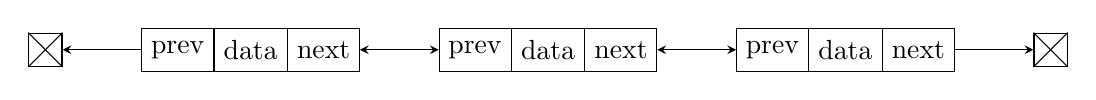
\begin{tikzpicture}[list/.style={rectangle split, rectangle split parts=3,
					draw, rectangle split horizontal}, >=stealth, start chain]
		\node[on chain,draw,inner sep=6pt] (NULL1) {};
		\node[list,on chain] (A) {prev \nodepart{second} data \nodepart{third} next};
		\node[list,on chain] (B) {prev \nodepart{second} data \nodepart{third} next};
		\node[list,on chain] (C) {prev \nodepart{second} data \nodepart{third} next};
		\node[on chain,draw,inner sep=6pt] (NULL2) {};
		\draw (NULL1.north east) -- (NULL1.south west);
		\draw (NULL1.north west) -- (NULL1.south east);
		\draw (NULL2.north east) -- (NULL2.south west);
		\draw (NULL2.north west) -- (NULL2.south east);
		\draw[<-] let \p1 = (A.west), \p2 = (A.center) in (NULL1) -- (\x1,\y2);
		\draw[<->] let \p1 = (A.east), \p2 = (A.center) in (\x1,\y2) -- (B);
		\draw[<->] let \p1 = (B.east), \p2 = (B.center) in (\x1,\y2) -- (C);
		\draw[->] let \p1 = (C.east), \p2 = (C.center) in (\x1,\y2) -- (NULL2);
	\end{tikzpicture}
	\caption{双向链表}
\end{figure}

\begin{table}[H]
	\centering
	\setlength{\tabcolsep}{5mm}{
		\begin{tabular}{|l|l|}
			\hline
			\textbf{操作}      & \textbf{功能}         \\
			\hline
			list<T> lst        & 创建空的list          \\
			\hline
			list<T> lst(n)     & 创建含有n个元素的list \\
			\hline
			list<T> lst1(lst2) & 使用lst2初始化lst1    \\
			\hline
			lst.size()         & 返回list元素个数      \\
			\hline
			lst.clear()        & 删除所有元素          \\
			\hline
			lst.empty()        & 判断list是否为空      \\
			\hline
			lst.front()        & 返回第一个元素        \\
			\hline
			lst.back()         & 返回最后一个元素      \\
			\hline
			lst.insert()       & 插入一个元素          \\
			\hline
			lst.erase()        & 删除一个元素          \\
			\hline
			lst.push\_front()  & 在头部添加一个元素    \\
			\hline
			lst.push\_back()   & 在尾部添加一个元素    \\
			\hline
			lst.pop\_front()   & 删除第一个元素        \\
			\hline
			lst.pop\_back()    & 删除最后一个元素      \\
			\hline
			lst.remove()       & 删除元素              \\
			\hline
			lst.reverse()      & 反转list              \\
			\hline
			lst.sort()         & 排序                  \\
			\hline
			lst.unique()       & 去除相邻的重复元素    \\
			\hline
			lst.merge()        & 合并两个有序list      \\
			\hline
		\end{tabular}
	}
	\caption{list操作}
\end{table}

其中,lst.unique()并不是把重复的元素删除,而是全部放到数组尾部,返回去重后的尾地址。unique()中不自带sort(),因此需要先使用sort()进行排序。 \\

\mybox{list}

\begin{lstlisting}[language=C++]
#include <iostream>
#include <list>

using namespace std;

void printList(list<int> lst) {
    for(list<int>::iterator iter = lst.begin();
                            iter != lst.end();
                            iter++) {
        cout << *iter << " ";
    }
    cout << endl;
}

int main() {
    list<int> lst;

    lst.push_back(11);       // [11]
    lst.push_front(22);      // [22, 11]
    cout << lst.front() << endl;    // 22
    cout << lst.back() << endl;     // 11

    lst.insert(++lst.begin(), 3);   // [22, 3, 11]
    lst.insert(--lst.end(), 2);     // [22, 3, 2, 11]
    lst.push_back(2);               // [22, 3, 2, 11, 2]
    printList(lst);

    lst.pop_front();                // [3, 2, 11, 2]
    lst.sort();                     // [2, 2, 3, 11]
    lst.unique();                   // [2, 3, 11]
    printList(lst);

    lst.sort();                     // [2, 3, 11]
    printList(lst);

    list<int> lst2{1, 2, 8};
    lst.merge(lst2);                // [1, 2, 2, 3, 8, 11]
    printList(lst);

    return 0;
}
\end{lstlisting}

\begin{tcolorbox}
	\mybox{运行结果}
	\begin{verbatim}
22
11
22 3 2 11 2
2 3 11
2 3 11
1 2 2 3 8 11
	\end{verbatim}
\end{tcolorbox}

\subsection{forward\_list}

forward\_list和list的区别在于前者是单向链表,每个元素内部只有一个链接指向下一个元素,因此在存储方面list会消耗更多的空间。 \\

\begin{figure}[H]
	\centering
	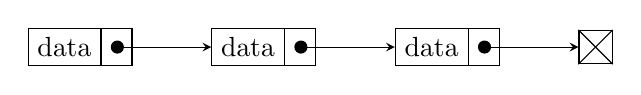
\begin{tikzpicture}[list/.style={rectangle split, rectangle split parts=2,
					draw, rectangle split horizontal}, >=stealth, start chain]
		\node[list,on chain] (A) {data};
		\node[list,on chain] (B) {data};
		\node[list,on chain] (C) {data};
		\node[on chain,draw,inner sep=6pt] (D) {};
		\draw (D.north east) -- (D.south west);
		\draw (D.north west) -- (D.south east);
		\draw[*->] let \p1 = (A.two), \p2 = (A.center) in (\x1,\y2) -- (B);
		\draw[*->] let \p1 = (B.two), \p2 = (B.center) in (\x1,\y2) -- (C);
		\draw[*->] let \p1 = (C.two), \p2 = (C.center) in (\x1,\y2) -- (D);
	\end{tikzpicture}
	\caption{单向链表}
\end{figure}

forward\_list不支持反向迭代器,并且没有指向尾元素的迭代器,因此不提供back()、push\_back()、pop\_back()等操作。

\newpage

\section{容器适配器}

\subsection{stack}

栈,又名堆栈,是一种运算受限的线性数据结构,栈只能在表尾进行插入和删除操作。 \\

栈中的元素只能先进后出(FILO, First In Last Out)。最早进入栈的元素所存放的位置叫作栈底(bottom),最后进入栈的元素存放的位置叫作栈顶(top)。 \\

\begin{figure}[H]
	\centering
	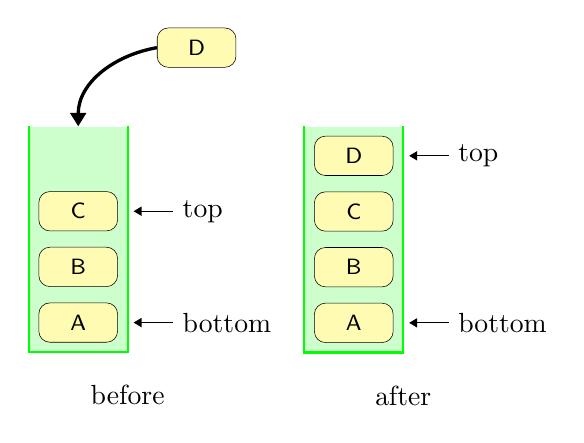
\begin{tikzpicture}
		\matrix[queue] (Q1) {
		|[fill=none, draw=none]| \\
		|(front)| C\\
		B\\
		|(rear)| A\\};
		\draw[green,thick,-] (Q1.north west) |-(Q1.south)-| (Q1.north east);
		\draw[<-] ([xshift=.2cm]front.east) -- ++ (0:.5) node[right] {top};
		\draw[<-] ([xshift=.2cm]rear.east) -- ++ (0:.5) node[right] {bottom};
		\draw[<-,very thick] (Q1.north) to[out=90,in=190] ++ (1,1) node[right, queue element] (D) {D};
		\node[below=3mm of Q1.south east] {before};

		\scope[xshift=3.5cm]
		\matrix[queue] (Q1) {
			|(front)| D \\
			C           \\
			B           \\
			|(rear)| A\\};
		\draw[green,thick,-] (Q1.north west) |-(Q1.south)-| (Q1.north east);
		\draw[<-] ([xshift=.2cm]front.east) -- ++ (0:.5) node[right] {top};
		\draw[<-] ([xshift=.2cm]rear.east) -- ++ (0:.5) node[right] {bottom};
		\node[below=3mm of Q1.south east] {after};
		\endscope
	\end{tikzpicture}
	\caption{栈}
\end{figure}

向一个栈插入新元素的操作称为入栈push(或进栈、压栈),从一个栈删除元素的操作称为出栈pop(或退栈、弹栈)。入栈操作就是把新元素放入栈中,只允许从栈顶一侧放入元素,新元素的位置将会成为新的栈顶。出栈操作就是把新元素从栈中弹出,只有栈顶元素才允许出栈,出栈元素的前一个元素将会成为新的栈顶。

\begin{table}[H]
	\centering
	\setlength{\tabcolsep}{5mm}{
		\begin{tabular}{|l|l|}
			\hline
			\textbf{操作} & \textbf{功能}                        \\
			\hline
			empty()       & 判断栈是否为空                       \\
			\hline
			size()        & 返回栈中元素个数                     \\
			\hline
			push()        & 入栈,调用底层容器的push\_back()实现 \\
			\hline
			pop()         & 出栈                                 \\
			\hline
			top()         & 返回栈顶元素的引用                   \\
			\hline
		\end{tabular}
	}
	\caption{stack操作}
\end{table}

\mybox{stack}

\begin{lstlisting}[language=C++]
#include <iostream>
#include <stack>

using namespace std;

int main() {
	stack<int> s;
	s.push(1);
	s.push(2);
	s.push(3);
	cout << s.top() << endl;

	while(!s.empty()) {
		cout << s.top() << endl;
		s.pop();
	}
	return 0;
}
\end{lstlisting}

\begin{tcolorbox}
	\mybox{运行结果}
	\begin{verbatim}
3
3
2
1
	\end{verbatim}
\end{tcolorbox}

\subsection{deque}

deque双端队列是一种同时具有队列和栈的性质的数据结构,双端队列可以从其两端插入和删除元素。

\begin{figure}[H]
	\centering
	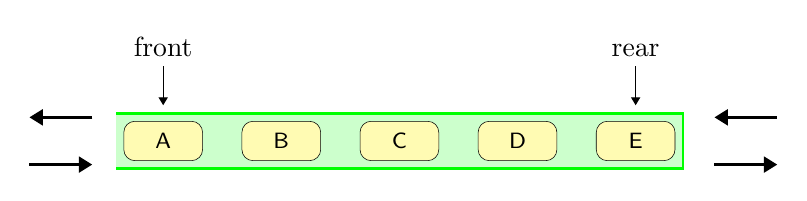
\begin{tikzpicture}
		\fill[green!20] (6.6,.35) rectangle (-.6,-.35);
		\draw[green,thick] (-.6,.35) -- (6.6,.35) |- (-.6,-.35);
		\foreach \i/\name in {0/A,1/B,2/C,3/D,4/E}
		\node[queue element] (\name) at (1.5*\i,0) {\name};
		\draw[<-] ([yshift=.2cm]E.north) -- ++ (0,.5) node[above] {rear};
		\draw[<-] ([yshift=.2cm]A.north) -- ++ (0,.5) node[above] {front};

		\draw[->,very thick] (-0.9,0.3) -- (-1.7,0.3);
		\draw[->,very thick] (-1.7,-0.3) --  (-0.9,-0.3);

		\draw[<-,very thick] (7,0.3) -- (7.8,0.3);
		\draw[<-,very thick] (7.8,-0.3) -- (7,-0.3);
	\end{tikzpicture}
	\caption{双端队列}
\end{figure}

\begin{table}[H]
	\centering
	\setlength{\tabcolsep}{5mm}{
		\begin{tabular}{|l|l|}
			\hline
			\textbf{操作} & \textbf{功能}       \\
			\hline
			empty()       & 判断deque是否为空   \\
			\hline
			size()        & 返回deque中元素个数 \\
			\hline
			front()       & 返回首元素引用      \\
			\hline
			back()        & 返回尾元素引用      \\
			\hline
			push\_front() & 在头部添加一个元素  \\
			\hline
			push\_back()  & 在尾部添加一个元素  \\
			\hline
			pop\_front()  & 在头部删除一个元素  \\
			\hline
			pop\_back()   & 在尾部删除一个元素  \\
			\hline
			clear()       & 清空deque           \\
			\hline
		\end{tabular}
	}
	\caption{deque操作}
\end{table}

\mybox{deque}

\begin{lstlisting}[language=C++]
#include <iostream>
#include <deque>

using namespace std;

int main() {
	deque<int> deq;
	
	deq.push_front(1);
	deq.push_front(2);
	deq.push_back(3);
	deq.push_back(4);
	cout << deq.front() << endl;
	cout << deq.back() << endl;

	deq.pop_back();
	deq.pop_front();
	cout << deq.front() << endl;
	cout << deq.back() << endl;

	return 0;
}
\end{lstlisting}

\begin{tcolorbox}
	\mybox{运行结果}
	\begin{verbatim}
2
4
1
3
	\end{verbatim}
\end{tcolorbox}

\subsection{priority\_queue}

普通的队列是一种先进先出(FIFO, First In First Out)的数据结构,元素在队尾添加,在队头删除。 \\

在优先队列priority\_queue中,元素被赋予优先级,当访问元素时,具有最高优先级的元素最先被访问。使用priority\_queue需要包含头文件<queue>。

\begin{table}[H]
	\centering
	\setlength{\tabcolsep}{5mm}{
		\begin{tabular}{|l|l|}
			\hline
			\textbf{操作} & \textbf{功能}      \\
			\hline
			empty()       & 判断队列是否为空   \\
			\hline
			size()        & 返回队列中元素个数 \\
			\hline
			top()         & 访问队头           \\
			\hline
			push()        & 插入元素           \\
			\hline
			pop()         & 弹出队头           \\
			\hline
		\end{tabular}
	}
	\caption{priority\_queue操作}
\end{table}

\mybox{priority\_deque}

\begin{lstlisting}[language=C++]
#include <iostream>
#include <queue>

using namespace std;

int main() {
	priority_queue<int> pq;
	pq.push(9);
	pq.push(2);
	pq.push(8);

	while(!pq.empty()) {
		cout << pq.top() << endl;
		pq.pop();
	}
	return 0;
}
\end{lstlisting}

\begin{tcolorbox}
	\mybox{运行结果}
	\begin{verbatim}
9
8
2
	\end{verbatim}
\end{tcolorbox}

\newpage

\section{关联容器}

\subsection{关联容器}

顺序容器的元素是按照在容器中的位置来保存和访问的,关联容器的元素按照关键字来保存和访问。关联容器支持高效地关键字查询和访问。所有关联容器都支持通用容器操作,但不支持顺序容器特有的操作,例如push\_front()或push\_back()。 \\

set和map是两种关联容器,set中的元素只包含关键字,而map中的元素是键值对(key-value pair)。

\begin{table}[H]
	\centering
	\setlength{\tabcolsep}{3mm}{
		\begin{tabular}{|l|l|l|}
			\hline
			\textbf{关联容器}   & \textbf{描述}               & \textbf{头文件}  \\
			\hline
			set                 & 只保存关键字的容器          & <set>            \\
			\hline
			multiset            & 关键字可以重复出现的set     & <set>            \\
			\hline
			unordered\_set      & 用哈希函数组织的set         & <unordered\_set> \\
			\hline
			unordered\_multiset & 哈希组织的set,关键字可重复 & <unordered\_set> \\
			\hline
			map                 & 保存键值对的容器            & <map>            \\
			\hline
			multimap            & 关键字可重复出现的map       & <map>            \\
			\hline
			unordered\_map      & 用哈希函数组织的map         & <unordered\_map> \\
			\hline
			unordered\_multimap & 哈希组织的map,关键字可重复 & <unordered\_map> \\
			\hline
		\end{tabular}
	}
	\caption{关联容器}
\end{table}

set是关键字的集合,其底层实现使用的是红黑树,当想要查找一个值是否存在时可以使用。set是模板,使用时必须在模板参数中指定元素类型。 \\

map是模板,使用时必须在模板参数中指定key和value的类型。map常称为关联数组或字典,但是其下标不必是整数,而是通过关键字来查找值。 \\

map的元素都是pair类型,pair也是模板,定义在<utility>中,一个pair保存两个public的数据成员,分别叫first和second。 \\

\mybox{关键词提取}

\begin{lstlisting}[title=summary.txt, breaklines=true, breakatwhitespace=false]
Internet of Things allows billions of physical objects to 
be connected to collect and exchange data for offering various 
applications, such as environmental monitoring, infrastructure 
management, and home automation. On the other hand, IoT has 
unsupported features that are critical for some IoT applications, 
including smart traffic lights, home energy management and 
augmented reality. To support these features, fog computing is 
integrated into IoT to extend computing, storage and networking 
resources to the network edge. Unfortunately, it is confronted 
with various security and privacy risks, which raise serious 
concerns towards users.
\end{lstlisting}

\begin{lstlisting}[title=excludes.txt]
the a an is this
that of at in on for
and it with to we I
into which these those are
be as has have or
\end{lstlisting}

\begin{lstlisting}[language=C++, title=STL\_set\_map.cpp]
#include <iostream>
#include <fstream>
#include <sstream>
#include <string>
#include <vector>
#include <set>
#include <map>
#include <cctype>
#include <algorithm>

using namespace std;

string getSummary(string filename) {
	ifstream in(filename);
	string summary;
	string line;
	while (getline(in, line)) {
		summary += line;
	}
	in.close();
	return summary;
}

set<string> getExcludes(string filename) {
	ifstream in(filename);
	set<string> excludes;
	string token;
	while (in >> token) {
		excludes.insert(token);
	}
	in.close();
	return excludes;
}

int main() {
	string summary = getSummary("summary.txt");
	vector<string> tokens;

	istringstream in(summary);
	string token;
	while (in >> token) {
		// eliminate the trailing punctuation
		if (!isalpha(token.back())) {
			token.pop_back();
		}

		// convert to lower case
		transform(
			token.begin(), token.end(),
			token.begin(), ::tolower);

		tokens.push_back(token);
	}

	set<string> excludes = getExcludes("excludes.txt");
	map<string, int> keywords;

	for (string token : tokens) {
		// not in excludes set
		if (excludes.find(token) == excludes.end()) {
			keywords[token]++;
		}
	}

	for (auto& p : keywords) {
		// print keywords that appear more than once
		if (p.second > 1) {
			cout << p.first << ": " << p.second << endl;
		}
	}

	return 0;
}
\end{lstlisting}

\begin{tcolorbox}
	\mybox{运行结果}
	\begin{verbatim}
applications: 2
computing: 2
features: 2
home: 2
iot: 3
management: 2
various: 2
	\end{verbatim}
\end{tcolorbox}

\newpage

\section{泛型算法}

\subsection{泛型算法(Generic Algorithm)}

标准库未给容器添加大量功能,而是提供一组独立于容器的泛型算法。它们实现了一些经典算法的公共接口,可用于不同类型的容器和元素。标准库算法不直接操作容器,而是遍历两个迭代器指定的元素范围。指针类似于内置数组上的迭代器,故泛型算法也可操作内置数组和指针。 \\

大多数算法定义在<algorithm>中,另外一组数值算法定义在<numeric>中。 \\

大多标准库算法都对一个范围内的元素操作,这个范围称为输入范围,接受输入范围的算法总是用前两个参数来表示输入范围。多数算法遍历输入范围的方式相似,但使用元素的方法不同,如是否读、是否写、是否重排等。 \\

\subsection{只读算法}

只读算法只读取输入范围的元素,但不改变它们。使用只读算法,最好用cbegin()和cend()。 \\

find()的作用是将范围中每一个元素与给定值比较,返回第一个等于给定值的元素的迭代器,如果没有匹配则返回该范围的尾后迭代器。find()会调用给定值类型的【==】运算符来比较。

\vspace{-0.5cm}

\begin{lstlisting}[language=C++]
template <class InputIterator, class T>
InputIterator find(
	InputIterator first, InputIterator last, const T& val
);
\end{lstlisting}

count()的作用是将范围中每一个元素与给定值比较,返回给定值在范围中出现的次数。 \\

accumulate()定义于<numeric>,其作用是对范围中元素求和,再加上给定值,返回求值结果。accumulate()会调用给定值类型的【+】运算符来求和。

\vspace{-0.5cm}

\begin{lstlisting}[language=C++]
template <class InputIterator, class T>
T accumulate(InputIterator first, InputIterator last, T init);
\end{lstlisting}

equal()的作用是确定两个序列的值是否相同,若果所有元素都相等时返回true,否则false。函数接受有3个参数,前两个是第一个序列的输入范围,第三个参数是第二个范围的首迭代器。equal()会调用【==】运算符来比较,元素类型不必严格一致。

\vspace{-0.5cm}

\begin{lstlisting}[language=C++]
template <class InputIterator1, class InputIterator2>
bool equal(
	InputIterator1 first1, InputIterator1 last1, 
	InputIterator2 first2
);
\end{lstlisting}

\vspace{0.5cm}

\mybox{只读算法}

\begin{lstlisting}[language=C++]
#include <iostream>
#include <vector>
#include <algorithm>
#include <numeric>

using namespace std;

int main() {
	vector<int> v1 = {40, 9, 20, 34, 7, 34, 85, 9};
	vector<int> v2 = {40, 9, 20, 34, 7, 34, 85, 9};
	int key = 34;
	
	vector<int>::iterator iter = find(
		v1.begin(), v1.end(), key
	);
	if(iter != v1.end()) {
		cout << "key found in vector: " << *iter << endl;
	} else {
		cout << "key not found" << endl;
	}
	
	cout << key << " appears "
		 << count(v1.begin(), v1.end(), key) << endl;
	cout << "sum = "
		 << accumulate(v1.begin(), v1.end(), 0) << endl;
	cout << "v1 == v2? " << boolalpha
		 << equal(v1.begin(), v1.end(), v2.begin()) << endl;
		 
	return 0;
}
\end{lstlisting}

\begin{tcolorbox}
	\mybox{运行结果}
	\begin{verbatim}
key found in vector: 34
34 appears 2
sum = 238
v1 == v2? true
	\end{verbatim}
\end{tcolorbox}

\subsection{写容器元素算法}

写容器元素算法可对序列中元素重新赋值,要求原序列大小不小于要写入的元素数目。 \\

fill()的作用是用给定值填满输入范围,函数接受3个参数,前2个是输入范围,第3个是给定值。

\vspace{-0.5cm}

\begin{lstlisting}[language=C++]
template <class ForwardIterator, class T>
void fill(
	ForwardIterator first, ForwardIterator last, const T& val
);
\end{lstlisting}

copy()的作用是将输入范围的值拷贝到目标序列,返回目标序列的尾后迭代器。函数接受3个参数,前2个是输入范围,第3个是目标序列的起始位置。

\vspace{-0.5cm}

\begin{lstlisting}[language=C++]
template <class InputIterator, class OutputIterator>
OutputIterator copy(
	InputIterator first, InputIterator last,
	OutputIterator result
);
\end{lstlisting}

replace()的作用是将序列中所有等于给定值的元素换为另一个值,函数接受4个参数,前2个是输入范围,后2个分别是要搜索的值和新值。

\vspace{-0.5cm}

\begin{lstlisting}[language=C++]
template <class ForwardIterator, class T>
void replace(
	ForwardIterator first, ForwardIterator last, 
	const T& old_value, const T& new_value
);
\end{lstlisting}

\vspace{0.5cm}

\mybox{写容器元素算法}

\begin{lstlisting}[language=C++]
#include <iostream>
#include <vector>
#include <algorithm>

using namespace std;

ostream& operator<<(ostream& out, vector<int>& v) {
	for(vector<int>::iterator iter = v.begin(); 
	iter != v.end(); 
	iter++
	) {
		out << *iter << " ";
	}
	return out;
}

int main() {
	vector<int> v1 = {9, 2, 8, 8, 2, 1, 0, 1, 2};
	vector<int> v2(10);
	
	fill(v2.begin(), v2.end(), 0);
	cout << v2 << endl;

	copy(v1.begin(), v1.end(), v2.begin());
	cout << v2 << endl;

	replace(v2.begin(), v2.end(), 1, 7);
	cout << v2 << endl;
	return 0;
}
\end{lstlisting}

\begin{tcolorbox}
	\mybox{运行结果}
	\begin{verbatim}
0 0 0 0 0 0 0 0 0 0 
9 2 8 8 2 1 0 1 2 0
9 2 8 8 2 7 0 7 2 0
	\end{verbatim}
\end{tcolorbox}

\subsection{重排容器元素算法}

重排容器元素算法可对容器中元素重新排列顺序。 \\

sort()的作用是重排输入序列的元素使其有序,函数接受2个参数表示输入范围,函数会调用序列元素类型的【<】运算符。 \\

标准库允许在执行算法时用自定义操作代替默认算符,而不需要在类型中重载。

\vspace{-0.5cm}

\begin{lstlisting}[language=C++]
template <class RandomAccessIterator>
void sort(
	RandomAccessIterator first, RandomAccessIterator last
);

template <class RandomAccessIterator, class Compare>
void sort(
	RandomAccessIterator first, RandomAccessIterator last, 
	Compare comp
);
\end{lstlisting}

谓词(predicate)是一个可调用的表达式,其返回值(true / false)可用作条件。按照参数的数量分为一元谓词和二元谓词。接受谓词的算法用该谓词代替默认的算符来操作元素。 \\

unique()的作用是重排输入序列,消除相邻重复项,返回消除后的无相邻重复值的尾后迭代器。unique()不真正删除元素,只是将后面的不重复值前移来覆盖前面的重复值,真正删除元素需要使用容器操作。

\vspace{-0.5cm}

\begin{lstlisting}[language=C++]
template <class ForwardIterator>
ForwardIterator unique(
	ForwardIterator first, ForwardIterator last
);

template <class ForwardIterator, class BinaryPredicate>
ForwardIterator unique(
	ForwardIterator first, ForwardIterator last,
	BinaryPredicate pred
);
\end{lstlisting}

\vspace{0.5cm}

\mybox{重排容器元素算法}

\begin{lstlisting}[language=C++]
#include <iostream>
#include <string>
#include <vector>
#include <algorithm>

using namespace std;

ostream& operator<<(ostream& out, vector<string>& v) {
	for(vector<string>::iterator iter = v.begin();
								iter != v.end();
								iter++) {
		out << *iter << " ";
	}
	return out;
}

bool isLonger(const string& s1, const string& s2) {
	return s1.size() > s2.size();
}

int main() {
	vector<string> v = {
		"C++", "Java", "Python",
		"C++", "C", "JavaScript", 
		"Golang", "C++"
	};
	
	sort(v.begin(), v.end());
	cout << v << endl;
	
	sort(v.begin(), v.end(), isLonger);
	cout << v << endl;
	
	vector<string>::iterator endUnique = unique(
	v.begin(), v.end()
);
	v.erase(endUnique, v.end());
	cout << v << endl;
	return 0;
}
\end{lstlisting}

\begin{tcolorbox}
	\mybox{运行结果}
	\begin{verbatim}
C C++ C++ C++ Golang Java JavaScript Python 
JavaScript Golang Python Java C++ C++ C++ C
JavaScript Golang Python Java C++ C
	\end{verbatim}
\end{tcolorbox}

\end{document}